% =====================================================================
% IEEE Conference Paper — Cassava Leaf Disease Classification
% Authors: Ali Baki Türköz, Emre Öztürk (Özyeğin University, MSc CS)
% Course: CS523 — Computer Vision
%
% Compile with pdfLaTeX on Overleaf:
%   - Set TeX Live version to latest
%   - Main document type: pdfLaTeX
%   - Bibliography is BibTeX (filecontents block at top)
% =====================================================================

\documentclass[conference]{IEEEtran}
\IEEEoverridecommandlockouts

% ---------- Packages ----------
\usepackage[T1]{fontenc}
\usepackage[utf8]{inputenc}
\usepackage{lmodern}
\usepackage{cite}
\usepackage{amsmath,amssymb,amsfonts}
\usepackage{algorithmic}
\usepackage{graphicx}
\usepackage{textcomp}
\usepackage{xcolor}
\usepackage{booktabs}
\usepackage{multirow}
\usepackage{array}
\usepackage{url}
\usepackage{hyperref}
\hypersetup{
    colorlinks=true,
    linkcolor=black,
    citecolor=black,
    urlcolor=blue,
}

\def\BibTeX{{\rm B\kern-.05em{\sc i\kern-.025em b}\kern-.08em
    T\kern-.1667em\lower.7ex\hbox{E}\kern-.125emX}}

% =====================================================================
% Inline bibliography (so Overleaf needs only this single .tex file)
% =====================================================================
\begin{filecontents*}{references.bib}
@inproceedings{he2016resnet,
  author    = {He, Kaiming and Zhang, Xiangyu and Ren, Shaoqing and Sun, Jian},
  title     = {Deep Residual Learning for Image Recognition},
  booktitle = {Proceedings of the IEEE Conference on Computer Vision and Pattern Recognition (CVPR)},
  year      = {2016},
  pages     = {770--778}
}
@inproceedings{tan2019efficientnet,
  author    = {Tan, Mingxing and Le, Quoc V.},
  title     = {{EfficientNet}: Rethinking Model Scaling for Convolutional Neural Networks},
  booktitle = {Proceedings of the 36th International Conference on Machine Learning (ICML)},
  year      = {2019},
  pages     = {6105--6114}
}
@inproceedings{dosovitskiy2021vit,
  author    = {Dosovitskiy, Alexey and Beyer, Lucas and Kolesnikov, Alexander and Weissenborn, Dirk and Zhai, Xiaohua and Unterthiner, Thomas and Dehghani, Mostafa and Minderer, Matthias and Heigold, Georg and Gelly, Sylvain and Uszkoreit, Jakob and Houlsby, Neil},
  title     = {An Image is Worth 16x16 Words: Transformers for Image Recognition at Scale},
  booktitle = {International Conference on Learning Representations (ICLR)},
  year      = {2021}
}
@inproceedings{deng2009imagenet,
  author    = {Deng, Jia and Dong, Wei and Socher, Richard and Li, Li-Jia and Li, Kai and Fei-Fei, Li},
  title     = {{ImageNet}: A Large-Scale Hierarchical Image Database},
  booktitle = {IEEE Conference on Computer Vision and Pattern Recognition (CVPR)},
  year      = {2009},
  pages     = {248--255}
}
@article{mohanty2016plantdisease,
  author    = {Mohanty, Sharada P. and Hughes, David P. and Salath\'{e}, Marcel},
  title     = {Using Deep Learning for Image-Based Plant Disease Detection},
  journal   = {Frontiers in Plant Science},
  year      = {2016},
  volume    = {7},
  pages     = {1419}
}
@article{ferentinos2018,
  author    = {Ferentinos, Konstantinos P.},
  title     = {Deep Learning Models for Plant Disease Detection and Diagnosis},
  journal   = {Computers and Electronics in Agriculture},
  year      = {2018},
  volume    = {145},
  pages     = {311--318}
}
@article{barbedo2018,
  author    = {Barbedo, Jayme G. A.},
  title     = {Factors Influencing the Use of Deep Learning for Plant Disease Recognition},
  journal   = {Biosystems Engineering},
  year      = {2018},
  volume    = {172},
  pages     = {84--91}
}
@article{mwebaze2020cassava,
  author    = {Mwebaze, Ernest and Gebru, Timnit and Frome, Andrea and Nsumba, Solomon and Tusubira, Jeremy},
  title     = {{iCassava 2019} Fine-Grained Visual Categorization Challenge},
  journal   = {arXiv preprint arXiv:1908.02900},
  year      = {2019}
}
@inproceedings{akiba2019optuna,
  author    = {Akiba, Takuya and Sano, Shotaro and Yanase, Toshihiko and Ohta, Takeru and Koyama, Masanori},
  title     = {{Optuna}: A Next-Generation Hyperparameter Optimization Framework},
  booktitle = {Proceedings of the 25th ACM SIGKDD International Conference on Knowledge Discovery and Data Mining (KDD)},
  year      = {2019},
  pages     = {2623--2631}
}
@inproceedings{lin2017focal,
  author    = {Lin, Tsung-Yi and Goyal, Priya and Girshick, Ross and He, Kaiming and Doll\'{a}r, Piotr},
  title     = {Focal Loss for Dense Object Detection},
  booktitle = {Proceedings of the IEEE International Conference on Computer Vision (ICCV)},
  year      = {2017},
  pages     = {2980--2988}
}
@inproceedings{szegedy2016label,
  author    = {Szegedy, Christian and Vanhoucke, Vincent and Ioffe, Sergey and Shlens, Jon and Wojna, Zbigniew},
  title     = {Rethinking the {Inception} Architecture for Computer Vision},
  booktitle = {Proceedings of the IEEE Conference on Computer Vision and Pattern Recognition (CVPR)},
  year      = {2016},
  pages     = {2818--2826}
}
@inproceedings{loshchilov2019adamw,
  author    = {Loshchilov, Ilya and Hutter, Frank},
  title     = {Decoupled Weight Decay Regularization},
  booktitle = {International Conference on Learning Representations (ICLR)},
  year      = {2019}
}
@inproceedings{loshchilov2017sgdr,
  author    = {Loshchilov, Ilya and Hutter, Frank},
  title     = {{SGDR}: Stochastic Gradient Descent with Warm Restarts},
  booktitle = {International Conference on Learning Representations (ICLR)},
  year      = {2017}
}
@inproceedings{micikevicius2018mixed,
  author    = {Micikevicius, Paulius and Narang, Sharan and Alben, Jonah and Diamos, Gregory and Elsen, Erich and Garcia, David and Ginsburg, Boris and Houston, Michael and Kuchaiev, Oleksii and Venkatesh, Ganesh and Wu, Hao},
  title     = {Mixed Precision Training},
  booktitle = {International Conference on Learning Representations (ICLR)},
  year      = {2018}
}
@article{breiman2001randomforests,
  author    = {Breiman, Leo},
  title     = {Random Forests},
  journal   = {Machine Learning},
  year      = {2001},
  volume    = {45},
  number    = {1},
  pages     = {5--32}
}
@inproceedings{zhong2020randomerasing,
  author    = {Zhong, Zhun and Zheng, Liang and Kang, Guoliang and Li, Shaozi and Yang, Yi},
  title     = {Random Erasing Data Augmentation},
  booktitle = {Proceedings of the AAAI Conference on Artificial Intelligence},
  year      = {2020}
}

@misc{kaggle2020cassava,
  author       = {{Kaggle} and {Makerere University AI Lab}},
  title        = {{Cassava Leaf Disease Classification}},
  year         = {2020},
  howpublished = {Kaggle Competition},
  url          = {https://www.kaggle.com/competitions/cassava-leaf-disease-classification},
  note         = {Accessed: 2026-05-18}
}
@misc{kqu7cassava,
  author       = {{kqu7}},
  title        = {{Kaggle-Cassava-Leaf-Disease-Classification}},
  year         = {2021},
  howpublished = {GitHub repository},
  url          = {https://github.com/kqu7/Kaggle-Cassava-Leaf-Disease-Classification},
  note         = {Accessed: 2026-05-18}
}
@misc{kozodoi2021cassava,
  author       = {Kozodoi, Nikolai},
  title        = {{Kaggle Leaf Disease Classification}: top-1\% solution},
  year         = {2021},
  howpublished = {GitHub repository},
  url          = {https://github.com/kozodoi/Kaggle_Leaf_Disease_Classification},
  note         = {Accessed: 2026-05-18}
}
@inproceedings{fang2023imagenettransfer,
  author    = {Fang, Alex and Kornblith, Simon and Schmidt, Ludwig},
  title     = {Does Progress on {ImageNet} Transfer to Real-World Datasets?},
  booktitle = {Advances in Neural Information Processing Systems (NeurIPS) Datasets and Benchmarks Track},
  year      = {2023}
}

@misc{kaggle2020leaderboard,
  author       = {{Kaggle} and {Makerere University AI Lab}},
  title        = {{Cassava Leaf Disease Classification}: Leaderboard},
  year         = {2021},
  howpublished = {Kaggle Competition Leaderboard},
  url          = {https://www.kaggle.com/competitions/cassava-leaf-disease-classification/leaderboard},
  note         = {Accessed: 2026-05-18}
}
@misc{lizh0019cassava,
  author       = {{lizh0019}},
  title        = {{Cassava}: 1st Place Solution for Cassava Leaf Disease Classification},
  year         = {2021},
  howpublished = {GitHub repository},
  url          = {https://github.com/lizh0019/cassava},
  note         = {Accessed: 2026-05-18}
}
@misc{tomyanabe2021cassava,
  author       = {Yanabe, Tomohiro},
  title        = {{Cassava Leaf Disease Classification}: 3rd Place Solution},
  year         = {2021},
  howpublished = {GitHub repository},
  url          = {https://github.com/TomYanabe/Cassava-Leaf-Disease-Classification},
  note         = {Accessed: 2026-05-18}
}
@misc{krutpatel2021cassava,
  author       = {Patel, Krut},
  title        = {My Solution for Cassava Leaf Disease Classification},
  year         = {2021},
  howpublished = {Analytics Vidhya / Medium article},
  url          = {https://medium.com/analytics-vidhya/cassava-leaf-disease-classification-kaggle-competition-4407ed1a995d},
  note         = {Accessed: 2026-05-18}
}
@misc{devonstanfield2021cassava,
  author       = {Stanfield, Devon},
  title        = {{cassava-infer}},
  year         = {2021},
  howpublished = {Kaggle notebook},
  url          = {https://www.kaggle.com/code/devonstanfield/cassava-infer},
  note         = {Accessed: 2026-05-18}
}
@misc{vadimtimakin2021cassava,
  author       = {Timakin, Vadim and Zhdanov, Maksim and Tagiev, Emin},
  title        = {{Cassava-Leaf-Disease-Classification}: Competition Pipeline and Solution},
  year         = {2021},
  howpublished = {GitHub repository},
  url          = {https://github.com/vadimtimakin/Cassava-Leaf-Disease-Classification},
  note         = {Accessed: 2026-05-18}
}

\end{filecontents*}

% =====================================================================
% Title and Authors
% =====================================================================
\begin{document}

\title{Cassava Leaf Disease Classification}

\author{
\IEEEauthorblockN{Ali Baki Türköz}
\IEEEauthorblockA{Department of Computer Science \\
M.Sc.\ Program \\
Özyeğin University \\
Istanbul, Türkiye \\
baki.turkoz@ozu.edu.tr}
\and
\IEEEauthorblockN{Emre Öztürk}
\IEEEauthorblockA{Department of Computer Science \\
M.Sc.\ Program \\
Özyeğin University \\
Istanbul, Türkiye \\
emre.ozturk.46760@ozu.edu.tr}
}

\maketitle

% =====================================================================
% Abstract
% =====================================================================
\begin{abstract}
Plant disease detection affects crop yield and food security, and cassava diagnosis is difficult because several leaf diseases exhibit visually similar symptoms. This paper compares three families of image-classification approaches on the Cassava Leaf Disease Classification (CLDC) benchmark: classical raw-pixel baselines (SGD classifier, logistic regression, Extra Trees, and Random Forest), convolutional models (ResNet-50 and EfficientNet-B4), and a transformer model (ViT-B/16). Deep models are fine-tuned from ImageNet-pretrained weights under a reproducibility-oriented 3-fold stratified cross-validation protocol with early stopping, mixed-precision training, and class-weighting treated as a searchable option. An Optuna categorical search is followed by a fixed-configuration augmentation ablation. Across hyperparameter trials, ViT-B/16 attains the strongest macro-F1 ($0.7803 \pm 0.0105$), outperforming the best ResNet-50 ($0.7405 \pm 0.0169$) and EfficientNet-B4 ($0.7274 \pm 0.0123$), while classical baselines remain below $0.21$ macro-F1. With the best augmentation policy (\texttt{heavy\_combo}), the final ViT-B/16 model reaches macro-F1 $0.7921 \pm 0.0068$ and accuracy $0.8855 \pm 0.0040$, with the largest per-class gain ($+0.0282$ F1) on the rarest class.
\end{abstract}

\begin{IEEEkeywords}
plant disease classification, cassava leaf disease, convolutional neural networks, vision transformer, transfer learning, Optuna, hyperparameter optimization, data augmentation, class imbalance, ablation study.
\end{IEEEkeywords}

% =====================================================================
% Introduction
% =====================================================================
\section{Introduction}
\label{sec:intro}

Agriculture remains a key pillar of global food security, and crop diseases continue to account for substantial yield losses worldwide. Among staple crops cultivated in tropical regions, cassava (\emph{Manihot esculenta}) is particularly important: it provides a major source of carbohydrates for millions of producers in sub-Saharan Africa. However, cassava is highly susceptible to a number of viral, bacterial, and arthropod-mediated diseases, including Cassava Bacterial Blight (CBB), Cassava Brown Streak Disease (CBSD), Cassava Green Mite (CGM), and Cassava Mosaic Disease (CMD)~\cite{mwebaze2020cassava}. Early and accurate identification of these diseases is essential for limiting losses, yet expert-driven manual inspection is expensive, slow, and difficult to scale.

Computer-vision-based automated disease detection offers a practical alternative. Deep convolutional neural networks (CNNs) have produced strong results in plant-disease classification under controlled laboratory conditions~\cite{mohanty2016plantdisease,ferentinos2018}, but generalization to images taken with mobile phones in farmers' fields---under varying illumination, complex backgrounds, motion blur, and label noise---remains an open challenge~\cite{barbedo2018}. The Cassava Leaf Disease Classification (CLDC) dataset~\cite{mwebaze2020cassava}, released through a Kaggle competition, captures exactly these real-world difficulties. It contains roughly $21{,}397$ images across five classes and exhibits severe class imbalance, with the CMD class accounting for more than $61\%$ of the data while the rarest class (CBB) accounts for only about $5\%$.

Recent advances in computer vision have introduced two complementary directions worth investigating on this benchmark. On the convolutional side, EfficientNet~\cite{tan2019efficientnet} provides a principled compound-scaling rule that obtains higher accuracy than ResNet-style backbones~\cite{he2016resnet} at comparable parameter budgets. On the architectural side, the Vision Transformer (ViT)~\cite{dosovitskiy2021vit} demonstrates that pure self-attention models, when pretrained on large-scale data, can match or exceed convolutional models on image classification. Whether these gains transfer to a noisy, imbalanced, in-the-wild agricultural domain such as cassava is a question that motivates this study.

In parallel, training-protocol decisions---such as the choice of optimizer, learning-rate schedule, loss function, and data-augmentation strategy---are known to have a comparable or even larger impact on final performance than the choice of backbone~\cite{loshchilov2019adamw,loshchilov2017sgdr,lin2017focal}. In settings with strong class imbalance and limited annotated samples, principled hyperparameter search and careful augmentation design are therefore not optional. This study addresses these considerations directly through an Optuna-based~\cite{akiba2019optuna} categorical search over hyperparameters and an explicit augmentation ablation.

The main contributions of this work are the following:
\begin{itemize}
  \item We provide a controlled, reproducibility-oriented comparison of three deep-learning architectures (ResNet-50, EfficientNet-B4, ViT-B/16) on CLDC under a unified 3-fold stratified cross-validation protocol, with class-weight handling, mixed-precision training, early stopping, and seed determinism.
  \item We include classical machine-learning baselines (SGD classifier, logistic regression, Extra Trees, and Random Forest) operating on grayscale flattened pixels with Principal-Component-Analysis (PCA) dimensionality reduction, to quantify the gap between raw-pixel classifiers and deep models on this task.
  \item We perform a categorical hyperparameter search using the Optuna framework with a Tree-structured Parzen Estimator (TPE) sampler and a median pruner, jointly searching over learning rate, weight decay, batch size, optimizer, loss function (including focal and label-smoothed variants), and learning-rate scheduler.
  \item We perform a data-augmentation ablation covering baseline, single-component, composite, and combined policies, and we analyze class weighting as a categorical option inside the hyperparameter search rather than as a separate matched-pair experiment.
\end{itemize}

The remainder of this paper is organized as follows. Section~\ref{sec:related} reviews related work in plant-disease classification, transfer learning, and hyperparameter optimization. Section~\ref{sec:method} describes the methodology in detail, including the dataset, models, training protocol, hyperparameter search procedure, and ablation design. Section~\ref{sec:results} presents the experimental results, the augmentation ablation, and per-class analyses. Section~\ref{sec:discussion} concludes with a discussion of findings, limitations, and directions for future work.

% =====================================================================
% Related Work
% =====================================================================

\section{Related Work}
\label{sec:related}

\subsection{Plant-Disease Classification in the Wild}
Early image-based plant-disease studies demonstrated that deep CNNs can reach very high accuracy under controlled imaging conditions. Mohanty \emph{et al.}~\cite{mohanty2016plantdisease} trained AlexNet- and GoogLeNet-style models on PlantVillage and reported test accuracies above $99\%$, while Ferentinos~\cite{ferentinos2018} confirmed the strength of pretrained CNNs across multiple crop species. These results are important but not directly representative of deployment: Barbedo~\cite{barbedo2018} showed that background clutter, illumination changes, occlusion, and annotation noise can substantially degrade recognition performance. The Cassava Leaf Disease Classification (CLDC) benchmark~\cite{mwebaze2020cassava,kaggle2020cassava} is therefore a stricter test case: images are acquired by farmers using mobile devices, symptoms are visually similar across classes, and the class distribution is highly imbalanced.

\subsection{Architectures and Transfer Learning}
ResNet-50~\cite{he2016resnet} remains a standard transfer-learning baseline because residual connections make deep CNN optimization stable. EfficientNet~\cite{tan2019efficientnet} improves the accuracy--efficiency trade-off through compound scaling of depth, width, and input resolution. ViT~\cite{dosovitskiy2021vit} replaces convolutional locality with self-attention over image patches and can be competitive when initialized from large-scale pretraining such as ImageNet~\cite{deng2009imagenet}. However, recent evidence suggests that ImageNet progress does not always transfer monotonically to real-world datasets. Fang \emph{et al.}~\cite{fang2023imagenettransfer} evaluated ImageNet-pretrained models on practical datasets including CLDC and reported that, on Cassava Leaf Disease, EfficientNet-B4, MobileNet, and ViT obtained $89.5\%$, $89.4\%$, and $88.8\%$ accuracy respectively, while a stronger Kaggle ensemble reached $91.3\%$ on the private leaderboard. This motivates evaluating backbone choice jointly with task-specific training choices rather than assuming that a larger or newer architecture will dominate.

\subsection{Kaggle Competition Solutions and K-Fold Evaluation}
The Kaggle CLDC competition provides a useful external reference point because submissions are evaluated by accuracy on a hidden test set and the final private leaderboard is computed on approximately $69\%$ of that test set~\cite{kaggle2020leaderboard}. These numbers should not be interpreted as a direct replacement for our 3-fold cross-validation results, because many competition pipelines use larger ensembles, external 2019 cassava data, test-time augmentation (TTA), pseudo-labeling, relabeling, and leaderboard-driven model selection. They are nevertheless informative because the strongest public solutions identify which training strategies worked in the same data domain.

The documented first-place solution associated with \texttt{golddiggaz}/\texttt{lizh0019} used an ensemble of EfficientNet-B4, ResNeXt50, ViT, and MobileNet/CropNet-style components and reported roughly $91.3\%$ accuracy on both public and private leaderboards~\cite{lizh0019cassava}. The rank-2 leaderboard entry by Devon Stanfield achieved $0.9043$ private leaderboard accuracy in the available leaderboard snapshot, and the associated public inference notebook uses Google's TensorFlow Hub CropNet cassava classifier~\cite{devonstanfield2021cassava}. The third-place TomYanabe solution is particularly relevant to our study because it reports a 5-fold StratifiedKFold protocol, ViT-B/16 variants at multiple input resolutions, 2020+2019 data, and TTA; its final submission reports CV $0.9075$, public leaderboard $0.9075$, and private leaderboard $0.9028$~\cite{tomyanabe2021cassava}. Krut Patel's ninth-place solution used stratified k-fold validation, ResNeXt50-32x4d and EfficientNet-B4 with soft voting, and TTA, reaching $0.895$ accuracy on both public and private leaderboards~\cite{krutpatel2021cassava}. Kozodoi's top-1\% solution combined CNNs and Vision Transformers in a stacking ensemble and reports $91.06\%$ test accuracy while ranking 14th among roughly $3{,}900$ teams~\cite{kozodoi2021cassava}. The kqu7 silver-medal solution used 5-fold StratifiedKFold, minority-sample weighting, heavy augmentation, ResNeXt50, and several EfficientNet variants; its individual model CV accuracies were $0.893$--$0.898$, and its final ensemble with 8x TTA reached $90.11\%$ public and $90.01\%$ private leaderboard accuracy~\cite{kqu7cassava}. Finally, the vadimtimakin solution highlights the effect of relabeling and external data, reporting that soft relabeling increased EfficientNet-B4 CV from $0.899$ to $0.915$ and that the pipeline used 5-fold SWSL ResNeXt-101 predictions, 2019 data, Mendeley leaf images, MixUp/CutMix/FMix, and lightweight TTA~\cite{vadimtimakin2021cassava}.

Compared with these competition-oriented pipelines, our best post-augmentation single ViT-B/16 model reaches $88.55\% \pm 0.40\%$ accuracy and $0.7921 \pm 0.0068$ macro-F1 under 3-fold stratified cross-validation, without ensembling, TTA, pseudo-labeling, relabeling, or external data. The gap to the strongest Kaggle systems is therefore expected: the leading entries optimize a full competition stack, while this paper isolates the effects of backbone family, hyperparameters, class-imbalance handling, and augmentation under one reproducible protocol.

\subsection{Class Imbalance, Augmentation, and Optimization}
Class imbalance is central to CLDC because CMD dominates the training set while the rarest class contributes only about $5\%$ of the images. We therefore compare loss reweighting, focal loss~\cite{lin2017focal}, and label-smoothed cross-entropy~\cite{szegedy2016label}. Data augmentation is equally important for in-the-wild leaf images: geometric and photometric transforms model viewpoint and lighting variation, while Random Erasing~\cite{zhong2020randomerasing} simulates occlusion and irrelevant background regions. Hyperparameter interactions across optimizer, scheduler, loss, and regularization make manual selection unreliable, so we use Optuna~\cite{akiba2019optuna} with TPE search and median pruning. AdamW~\cite{loshchilov2019adamw}, SGDR/cosine scheduling~\cite{loshchilov2017sgdr}, and mixed-precision training~\cite{micikevicius2018mixed} are included to make the search computationally tractable. Classical linear and tree-based baselines, including Random Forests~\cite{breiman2001randomforests}, are retained as lower-bound references for raw-pixel feature pipelines.

% =====================================================================
% Method
% =====================================================================
\section{Methodology}
\label{sec:method}

\subsection{Dataset}
\label{ssec:data}
We use the Cassava Leaf Disease Classification (CLDC) dataset~\cite{mwebaze2020cassava} released through a Kaggle competition. The dataset comprises approximately $21{,}397$ field-acquired RGB images of cassava leaves, captured by farmers using mobile phones under uncontrolled illumination, varying backgrounds, partial occlusion, and varying image quality. Each image is labeled with one of five mutually exclusive classes. Fig.~\ref{fig:class_dist} reports the per-class image counts and proportions in the training metadata used in this work, and Fig.~\ref{fig:samples} shows one representative image from each class.

\begin{figure}[t]
\centering
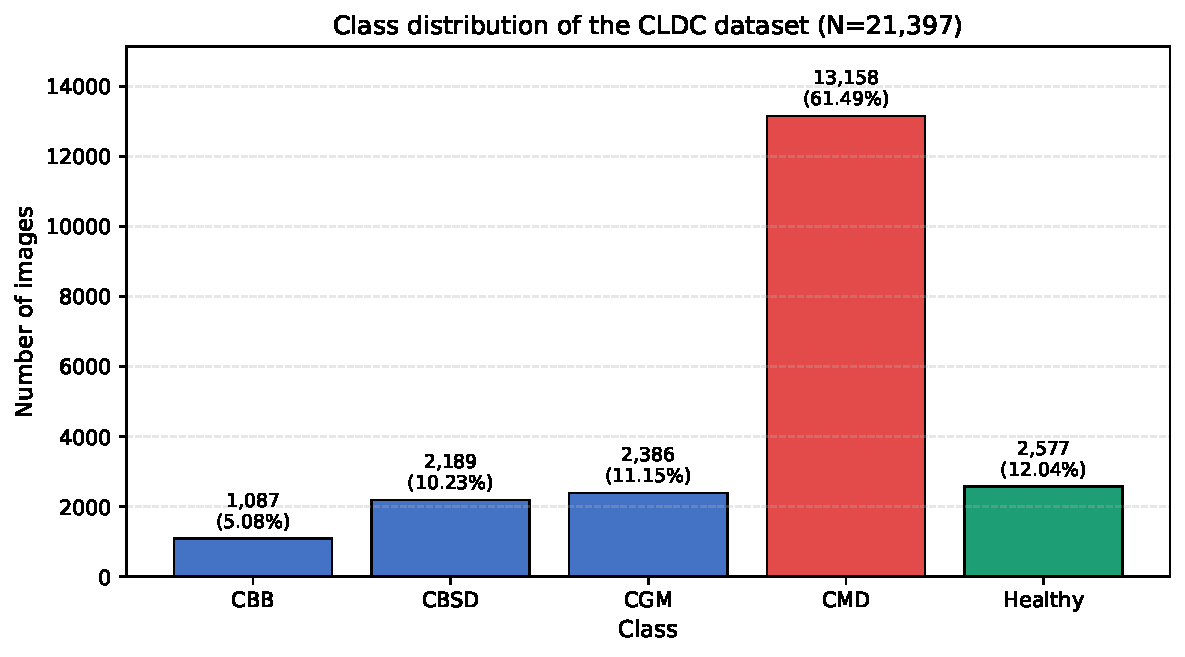
\includegraphics[width=\linewidth]{fig/fig_class_distribution.pdf}
\caption{Class distribution of the CLDC dataset used in this work. The Cassava Mosaic Disease (CMD) class accounts for $61.49\%$ of the data, while the rarest class (CBB) accounts for only $5.08\%$; the ratio between the largest and smallest classes is approximately $12{:}1$.}
\label{fig:class_dist}
\end{figure}

\begin{figure}[t]
\centering
\setlength{\tabcolsep}{2pt}
\begin{tabular}{ccccc}
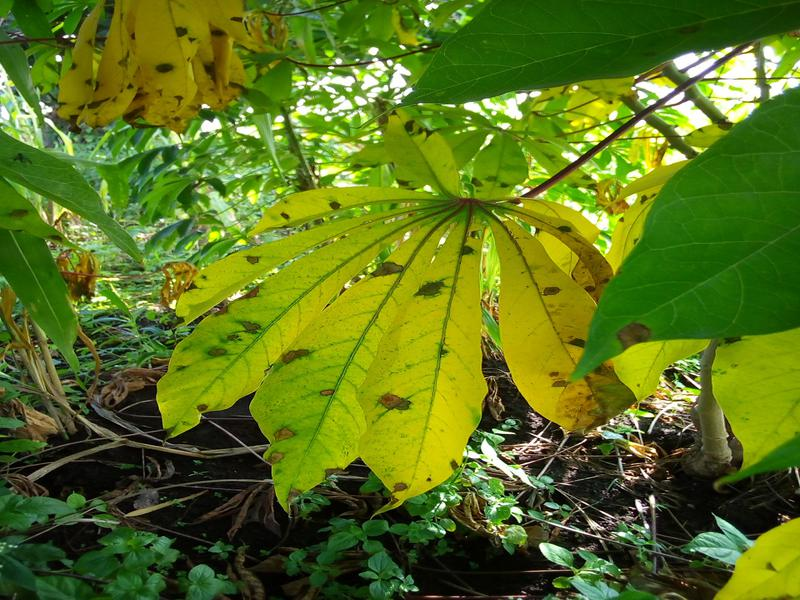
\includegraphics[width=0.165\linewidth]{fig/examples/label0_Cassava_Bacterial_Blight_CBB_2292154193.jpg} &
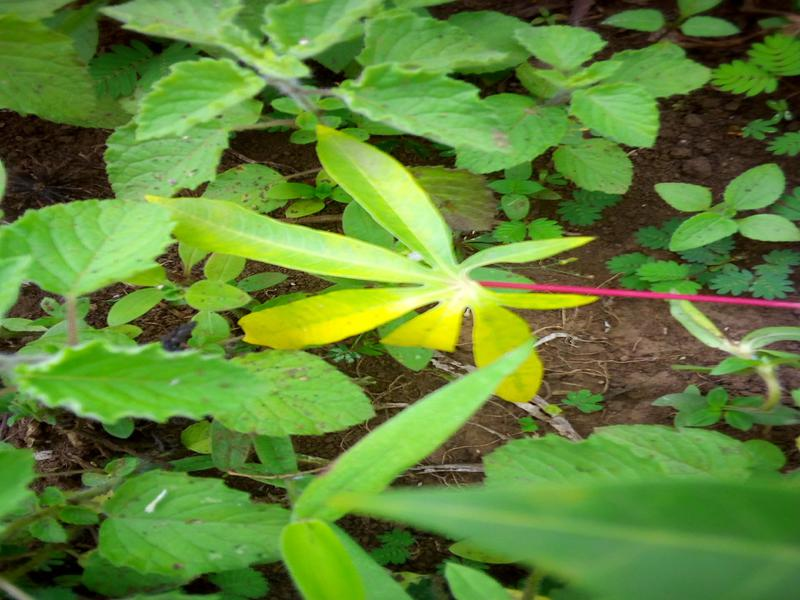
\includegraphics[width=0.165\linewidth]{fig/examples/label1_Cassava_Brown_Streak_Disease_CBSD_1053506407.jpg} &
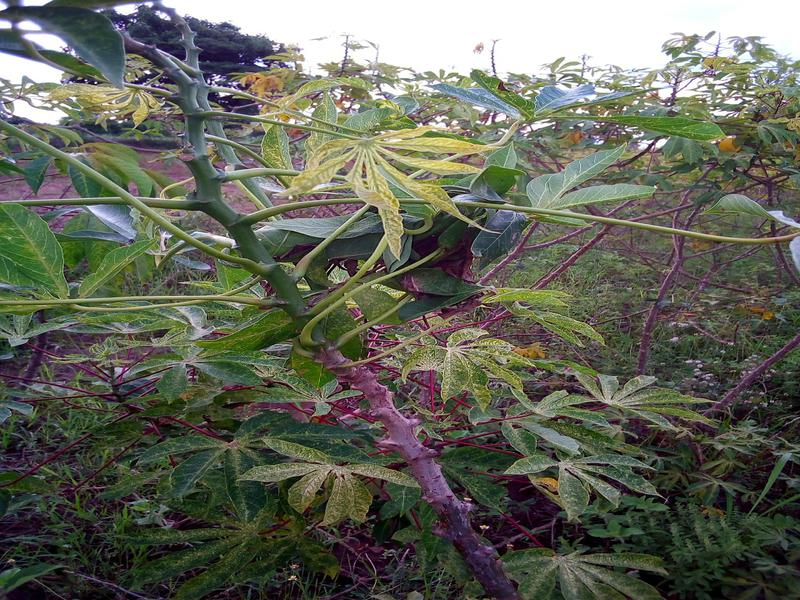
\includegraphics[width=0.165\linewidth]{fig/examples/label2_Cassava_Green_Mite_CGM_532304081.jpg} &
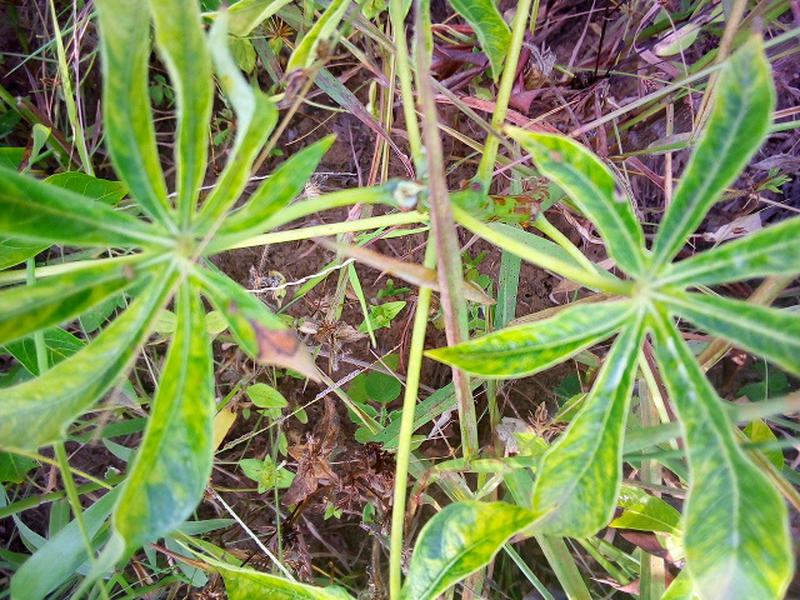
\includegraphics[width=0.165\linewidth]{fig/examples/label3_Cassava_Mosaic_Disease_CMD_575135832.jpg} &
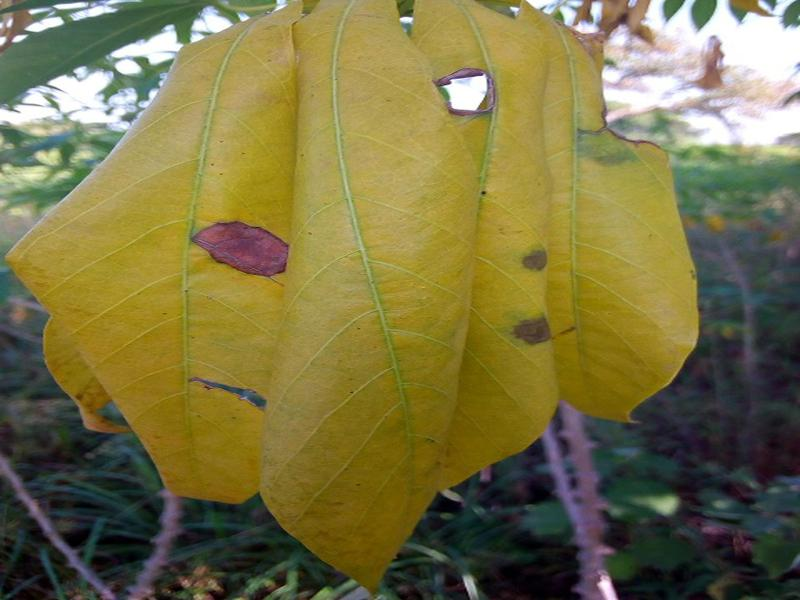
\includegraphics[width=0.165\linewidth]{fig/examples/label4_Healthy_1372417670.jpg} \\
\footnotesize CBB & \footnotesize CBSD & \footnotesize CGM & \footnotesize CMD & \footnotesize Healthy \\
\end{tabular}
\caption{Representative training images, one per class. The visual similarity between several disease classes, together with cluttered backgrounds and varying illumination, illustrates the difficulty of the CLDC benchmark.}
\label{fig:samples}
\end{figure}

The dataset is highly imbalanced: the CMD class alone accounts for $61.49\%$ of the training data, while the rarest class (CBB) accounts for only $5.08\%$. The ratio between the largest and smallest classes is approximately $12{:}1$. This imbalance, together with the in-the-wild acquisition conditions, motivates the class-weighting, focal-loss, and augmentation strategies described below.

\subsection{Evaluation Protocol}
\label{ssec:eval}
We use \emph{3-fold stratified cross-validation} as the sole evaluation protocol; no separate held-out test split is used. Stratification preserves the per-class proportions of Fig.~\ref{fig:class_dist} within each fold. For every experimental condition (every Optuna trial and every augmentation policy in the ablation), the full pipeline is repeated three times: training on two folds and evaluating on the held-out third. The reported metrics are the mean and standard deviation across the three folds. This corresponds to using out-of-fold validation predictions as a proxy for held-out test performance and provides a controlled alternative to a single fixed split.

For each fold, we record accuracy, macro-averaged precision, recall, and F1-score, the corresponding weighted-averaged metrics, and per-class precision, recall, and F1. We also record the full $5{\times}5$ confusion matrix and the training/validation loss and accuracy curves. Macro-averaged F1 (\texttt{f1\_macro}) is the primary metric used both as the Optuna objective and as the headline comparison criterion, because it weighs all classes equally and is therefore appropriate for the strongly imbalanced CLDC class distribution. Accuracy, in contrast, is dominated by the majority CMD class and is reported as a secondary metric only.

\subsection{Models}
\label{ssec:models}

\paragraph{Classical baselines}
For the classical pipeline, each image is converted to grayscale, resized to $64{\times}64$ pixels, scaled to $[0,1]$, and flattened to a $4{,}096$-dimensional feature vector. A single \texttt{StandardScaler} $\rightarrow$ \texttt{PCA(0.95 variance)} $\rightarrow$ classifier pipeline is then fit per fold. Four classifiers are evaluated: \texttt{sgd\_classifier}, \texttt{logistic\_regression}, \texttt{extra\_trees}, and \texttt{random\_forest}~\cite{breiman2001randomforests}. These baselines deliberately use a small input resolution and a single global feature representation; they are intended as a lower-bound reference, not as competitive solutions.

\paragraph{Deep models}
Three pretrained backbones are fine-tuned end-to-end. ResNet-50~\cite{he2016resnet} is loaded from \texttt{torchvision} with ImageNet-1k V2 weights; its final fully connected layer is replaced by a five-way classifier and the input resolution is set to $224{\times}224$. EfficientNet-B4~\cite{tan2019efficientnet} is loaded with ImageNet-1k weights; the final linear layer of its classifier head is replaced and the input resolution is also set to $224{\times}224$ to keep memory cost comparable. ViT-B/16~\cite{dosovitskiy2021vit} is loaded with ImageNet-1k weights and its classification head is replaced; following the architecture's design, the input resolution is set to $384{\times}384$. In all three cases, every parameter is set as trainable (no layer freezing); this corresponds to full fine-tuning.

\subsection{Training Protocol}
\label{ssec:training}

All deep models are trained with the same shared infrastructure, which differs only in the categorical hyperparameters chosen by Optuna. The base elements are the following.

\paragraph{Reproducibility}
A single global seed is set for Python's \texttt{random} module, NumPy, PyTorch (CPU and CUDA), and \texttt{PYTHONHASHSEED}. Deterministic cuDNN kernels are enabled, the cuBLAS workspace is configured for determinism, and PyTorch's \texttt{use\_deterministic\_algorithms} flag is activated. DataLoader workers are seeded individually. These settings produce deterministic-settings-based runs at the cost of modest throughput.

\paragraph{Mixed precision}
Training and inference are run under PyTorch's \texttt{torch.amp.autocast} with \texttt{float16} computation and a master copy of weights in \texttt{float32}, as introduced by Micikevicius \emph{et al.}~\cite{micikevicius2018mixed}. A \texttt{GradScaler} is used to prevent gradient underflow.

\paragraph{Class-imbalance handling}
For each training fold, per-class weights $w_c = N / (C \cdot n_c)$ are computed from the fold's label distribution, where $N$ is the number of training examples, $C=5$ is the number of classes, and $n_c$ is the count of class $c$. These weights are used either directly inside the loss (cross-entropy, label-smoothed cross-entropy, focal loss) or---in the unbalanced control condition---disabled. The \texttt{use\_class\_weights} flag is part of the ablation study described in Section~\ref{ssec:ablation}.

\paragraph{Loss functions}
We compare three loss families:
\begin{itemize}
  \item \emph{Cross-entropy}, optionally with class weights depending on the \texttt{use\_class\_weights} setting.
  \item \emph{Label-smoothed cross-entropy}~\cite{szegedy2016label} with smoothing parameter $\varepsilon \in \{0.05, 0.10, 0.20\}$.
  \item \emph{Focal loss}~\cite{lin2017focal} of the form
        $\mathrm{FL}(p_t) = -\alpha_t (1-p_t)^{\gamma} \log p_t$,
        with $\gamma \in \{1.0, 1.5, 2.0, 2.5\}$ and $\alpha_t$ taken from the class-balanced weights above.
\end{itemize}

\paragraph{Optimizers and schedulers}
The search space includes AdamW~\cite{loshchilov2019adamw}, Adam, and SGD with Nesterov momentum, with momentum $\in \{0.9, 0.95, 0.99\}$ where applicable. The learning-rate schedule is chosen from \texttt{ReduceLROnPlateau}, cosine annealing, and cosine annealing with warm restarts (SGDR)~\cite{loshchilov2017sgdr}. Plateau scheduling uses factor $0.5$ and patience $2$; cosine variants use $\eta_{\min}=10^{-7}$ and $T_0=5$ epochs with $T_{\text{mult}}=2$ for warm restarts.

\paragraph{Training loop, early stopping, and gradient clipping}
Each fold is trained for at most $200$ epochs with early stopping on validation loss (patience $20$). At the end of each epoch the best model state (lowest validation loss) is retained in memory; this state is restored before producing the fold's final predictions. Gradients are clipped to an $L_2$ norm of $1.0$ to stabilize fine-tuning of the larger ViT model.

\subsection{Hyperparameter Search with Optuna}
\label{ssec:optuna}

We use the Optuna framework~\cite{akiba2019optuna} with a Tree-structured Parzen Estimator (TPE) sampler and a median pruner. All hyperparameters are categorical so that the same search space can be reused across runs and inspected directly in the resulting trial logs. Table~\ref{tab:search_space} lists the search space. The Optuna objective is the mean macro-F1 across the three cross-validation folds of a trial; trials whose first-fold validation metric falls below the running median at the same epoch are pruned by the median pruner, allowing the budget to focus on promising configurations.

\begin{table}[t]
\centering
\caption{Optuna categorical search space for deep models.}
\label{tab:search_space}
\renewcommand{\arraystretch}{1.2}
\begin{tabular}{p{0.30\linewidth}p{0.60\linewidth}}
\toprule
\textbf{Hyperparameter} & \textbf{Candidate values} \\
\midrule
Model              & \texttt{resnet50}, \texttt{efficientnet\_b4}, \texttt{vit\_b\_16} \\
Learning rate      & $\{1{\times}10^{-5},\ 5{\times}10^{-5},\ 1{\times}10^{-4},\ 5{\times}10^{-4},\ 1{\times}10^{-3}\}$ \\
Weight decay       & $\{1{\times}10^{-5},\ 1{\times}10^{-4},\ 1{\times}10^{-3},\ 1{\times}10^{-2}\}$ \\
Batch size         & $\{16,\ 32,\ 64\}$ \\
Loss               & cross-entropy, label-smoothed CE, focal \\
Label smoothing    & $\{0.05,\ 0.10,\ 0.20\}$ (only for label-smoothed CE) \\
Focal $\gamma$     & $\{1.0,\ 1.5,\ 2.0,\ 2.5\}$ (only for focal loss) \\
Optimizer          & \texttt{adamw}, \texttt{adam}, \texttt{sgd} \\
SGD momentum       & $\{0.9,\ 0.95,\ 0.99\}$ (only for SGD) \\
Scheduler          & \texttt{plateau}, \texttt{cosine}, \texttt{cosine\_warm} \\
Class weighting    & $\{\text{enabled},\ \text{disabled}\}$ \\
\bottomrule
\end{tabular}
\end{table}

For every Optuna trial, the full 3-fold stratified cross-validation protocol of Section~\ref{ssec:eval} is executed and every fold-level and aggregate metric is logged to a single trial-indexed CSV file, together with the corresponding categorical configuration. The complete configuration of any reported result can therefore be reconstructed unambiguously from the trial log.

\subsection{Ablation Studies}
\label{ssec:ablation}

To isolate the effect of design choices that are especially relevant to CLDC, we conduct a fixed-configuration augmentation ablation and analyze class weighting as part of the Optuna search.

\paragraph{Augmentation ablation}
After the Optuna search has identified one of the best-performing hyperparameter configurations, this configuration is fixed and re-trained under different augmentation policies. Beyond the standard \emph{no-augmentation} baseline, the policies are grouped into single-component ablations (each of which isolates one transformation), composite recipes that combine a fixed set of standard transformations, and combined policies of varying intensity. Table~\ref{tab:aug_modes} summarizes the policies and what each one applies. All augmentation pipelines share the same final preprocessing step (resize, conversion to tensor, ImageNet normalization), so any performance differences are attributable to the augmentation policy alone.

\begin{table*}[t]
\centering
\caption{The $15$ augmentation settings evaluated in the augmentation ablation. All pipelines end with ImageNet normalization.}
\label{tab:aug_modes}
\renewcommand{\arraystretch}{1.15}
\begin{tabular}{p{0.16\linewidth}p{0.25\linewidth}p{0.53\linewidth}}
\toprule
\textbf{Category} & \textbf{Policy} & \textbf{Description} \\
\midrule
Baseline                       & \texttt{none}                         & Resize and normalize only; no augmentation. Reference for all other policies. \\
\midrule
\multirow{6}{*}{Single component}
                               & \texttt{flip\_only}                   & Horizontal/vertical flip and transpose only (spatial symmetry). \\
                               & \texttt{color\_only}                  & Color jitter and random grayscale only (no geometry). \\
                               & \texttt{contrast\_only}               & Contrast jitter only. \\
                               & \texttt{rotate\_only}                 & Rotation only (no flip, no crop). \\
                               & \texttt{blur\_noise\_light}           & Light Gaussian blur (sensor-noise simulation). \\
                               & \texttt{perspective\_light}           & Light perspective distortion (camera-tilt simulation). \\
\midrule
\multirow{3}{*}{Composite recipes}
                               & \texttt{comp\_resnext}                & RandomResizedCrop, Transpose, H/V flip, ShiftScaleRotate. \\
                               & \texttt{comp\_vit}                    & Above plus HSV jitter, brightness/contrast adjustments, CoarseDropout/Cutout. \\
                               & \texttt{comp\_3rd}                    & RandomResizedCrop, Transpose, H/V flip, ShiftScaleRotate only (minimal composite). \\
\midrule
\multirow{5}{*}{Combined}
                               & \texttt{heavy\_combo}                 & Full geometry + full color + Random Erasing. \\
                               & \texttt{cutout\_double}               & Double occlusion: Cutout + CoarseDropout. \\
                               & \texttt{regularization\_light\_combo} & Light crop + flip + small Random Erasing. \\
                               & \texttt{clahe\_enhanced}              & CLAHE histogram equalization with light color and geometry. \\
                               & \texttt{color\_light\_combo}          & Flip + ColorJitter; no geometric distortion. \\
\bottomrule
\end{tabular}
\end{table*}
\paragraph{Class weighting}
The \texttt{use\_class\_weights} flag is included in the Optuna search space as a categorical variable. Therefore, class-weighted and unweighted configurations are searched together, and the top-trial tables report both groups through the CW column. This design identifies whether class weighting survives model selection under the same search process; it is not treated as a separate matched-pair ablation with all other hyperparameters fixed.

\subsection{Logging Convention}
For every trial, a single row is appended to a master CSV file containing the full configuration (model, learning rate, weight decay, batch size, loss and its kwargs, optimizer and its kwargs, scheduler and its kwargs, augmentation policy, class-weighting flag, seed) and all aggregate and per-class metrics (mean and standard deviation across folds). Confusion matrices and training/validation curves are saved per trial. The reported metrics are taken from these experiment logs. Any language-editing assistance was restricted to grammar and readability polishing and did not generate or alter experimental results.

% =====================================================================
% Experimental Results
% =====================================================================
\section{Experimental Results}
\label{sec:results}

This section reports the results of the Optuna-driven hyperparameter search and the subsequent augmentation ablation. Hyperparameter trials were run for ResNet-50, EfficientNet-B4, and ViT-B/16 across class-weighted and unweighted configurations, and the classical baselines were evaluated under the same 3-fold stratified protocol. In addition, $15$ augmentation settings are evaluated on top of the selected best deep-learning configuration, including the no-augmentation reference.

\subsection{Classical Baselines}
Table~\ref{tab:results_ml} reports the results of the four classical machine-learning baselines (\texttt{sgd\_classifier}, \texttt{logistic\_regression}, \texttt{extra\_trees}, \texttt{random\_forest}) operating on grayscale $64{\times}64$ flattened pixels with StandardScaler and PCA ($95\%$ variance) preprocessing. Macro-F1 values stay below $0.21$ across all four methods, confirming that classical classifiers on raw global pixel statistics cannot capture the fine-grained leaf-texture cues that distinguish the five CLDC classes. Two effects are visible. First, tree-based methods (\texttt{extra\_trees}, \texttt{random\_forest}) achieve an apparently high accuracy ($\approx 0.6149$) only because they collapse to predicting the majority class CMD on almost every example: their macro-F1 of $0.1523$ is essentially the chance level for a single dominant prediction, and per-class precision and recall confirm this degenerate behavior. Second, linear models (\texttt{logistic\_regression}, \texttt{sgd\_classifier}) trade some accuracy for slightly better balance across classes, which raises macro-F1 marginally but is still far below any deep model. These results form a lower-bound reference for the deep-learning experiments that follow.

\begin{table*}[t]
\centering
\caption{Classical machine-learning baseline results on CLDC (3-fold stratified CV; raw $64{\times}64$ grayscale flatten $\rightarrow$ StandardScaler $\rightarrow$ PCA ($95\%$ variance) $\rightarrow$ classifier). All values are mean$\pm$std across the three folds.}
\label{tab:results_ml}
\renewcommand{\arraystretch}{1.25}
\setlength{\tabcolsep}{4pt}
\begin{tabular}{lcccc}
\toprule
\textbf{Classifier} & \textbf{F1 (macro)} & \textbf{Accuracy} & \textbf{Prec.\ (macro)} & \textbf{Recall (macro)} \\
\midrule
\texttt{sgd\_classifier} & $0.2012 \pm 0.0064$ & $0.3088 \pm 0.0145$ & 0.2133 & 0.2216 \\
\texttt{logistic\_regression} & $0.1898 \pm 0.0037$ & $0.2428 \pm 0.0043$ & 0.2167 & 0.2270 \\
\texttt{extra\_trees} & $0.1523 \pm 0.0000$ & $0.6149 \pm 0.0001$ & 0.1230 & 0.2000 \\
\texttt{random\_forest} & $0.1523 \pm 0.0000$ & $0.6149 \pm 0.0000$ & 0.1230 & 0.2000 \\
\bottomrule
\end{tabular}
\end{table*}


\subsection{Convolutional Models}
Table~\ref{tab:results_cnn} reports the top-10 ResNet-50 and EfficientNet-B4 trials, ranked by macro-F1. The best ResNet-50 trial reaches macro-F1 $0.7405 \pm 0.0169$ with accuracy $0.8521 \pm 0.0085$, an improvement of more than $0.54$ macro-F1 points over the best classical baseline. Nine of the top ten CNN trials use ResNet-50; the best EfficientNet-B4 trial appears at rank $9$ with macro-F1 $0.7274 \pm 0.0123$, indicating that on this dataset and at the budgets explored by Optuna, the larger compound-scaled architecture does not consistently outperform the simpler ResNet baseline. The top six CNN trials, and nine of the top ten overall, were trained without explicit class-balanced loss weighting (CW column ``$\times$''); the only class-weighted entry in the top ten is at rank $7$, which is consistent with the well-known difficulty of jointly tuning a class-reweighted loss and a strong optimizer on a strongly imbalanced classification problem.

\begin{table*}[t]
\centering
\caption{Top-10 CNN trials (ResNet-50 and EfficientNet-B4) on CLDC, ranked by macro-F1 over a 3-fold stratified CV. ``CW'' indicates whether class-balanced loss weighting was used. Values are mean$\pm$std across folds.}
\label{tab:results_cnn}
\renewcommand{\arraystretch}{1.2}
\setlength{\tabcolsep}{4pt}
\begin{tabular}{clccccc}
\toprule
\textbf{Rank} & \textbf{Model} & \textbf{CW} & \textbf{F1 (macro)} & \textbf{Accuracy} & \textbf{Prec.\ (macro)} & \textbf{Recall (macro)} \\
\midrule
1 & \texttt{resnet50} & $\times$ & $0.7405 \pm 0.0169$ & $0.8521 \pm 0.0085$ & 0.7576 & 0.7298 \\
2 & \texttt{resnet50} & $\times$ & $0.7375 \pm 0.0161$ & $0.8508 \pm 0.0081$ & 0.7530 & 0.7290 \\
3 & \texttt{resnet50} & $\times$ & $0.7345 \pm 0.0064$ & $0.8458 \pm 0.0040$ & 0.7400 & 0.7311 \\
4 & \texttt{resnet50} & $\times$ & $0.7311 \pm 0.0104$ & $0.8459 \pm 0.0046$ & 0.7445 & 0.7210 \\
5 & \texttt{resnet50} & $\times$ & $0.7310 \pm 0.0080$ & $0.8421 \pm 0.0059$ & 0.7353 & 0.7298 \\
6 & \texttt{resnet50} & $\times$ & $0.7303 \pm 0.0125$ & $0.8454 \pm 0.0059$ & 0.7434 & 0.7213 \\
7 & \texttt{resnet50} & \checkmark & $0.7299 \pm 0.0161$ & $0.8365 \pm 0.0171$ & 0.7197 & 0.7502 \\
8 & \texttt{resnet50} & $\times$ & $0.7281 \pm 0.0128$ & $0.8416 \pm 0.0090$ & 0.7370 & 0.7248 \\
9 & \texttt{efficientnet\_b4} & $\times$ & $0.7274 \pm 0.0123$ & $0.8494 \pm 0.0059$ & 0.7514 & 0.7112 \\
10 & \texttt{resnet50} & $\times$ & $0.7271 \pm 0.0094$ & $0.8415 \pm 0.0045$ & 0.7357 & 0.7254 \\
\bottomrule
\end{tabular}
\end{table*}


\subsection{Vision Transformer}
Table~\ref{tab:results_vit} reports the top-10 ViT-B/16 trials. ViT clearly outperforms both CNN backbones: every entry in the top-10 is above $0.7700$ macro-F1, the best trial achieves macro-F1 $0.7803 \pm 0.0105$ and accuracy $0.8792 \pm 0.0069$, and trial ranked $3$ achieves the highest accuracy overall ($0.8802 \pm 0.0070$). The gap to the best CNN trial is approximately $+0.04$ macro-F1 ($\approx 5\%$ relative improvement), which is a substantial margin given the difficulty of the dataset. As with the CNN results, the top ViT trials are dominated by unweighted training (eight of ten), while the two class-weighted entries at ranks $5$ and $8$ achieve slightly higher recall ($0.7930$ and $0.7911$) at the cost of lower precision, indicating that class weighting on this task trades minority-class recall for majority-class precision rather than improving the macro objective monotonically.

\begin{table*}[t]
\centering
\caption{Top-10 Vision Transformer (ViT-B/16) trials on CLDC, ranked by macro-F1 over a 3-fold stratified CV. ``CW'' indicates whether class-balanced loss weighting was used. Values are mean$\pm$std across folds.}
\label{tab:results_vit}
\renewcommand{\arraystretch}{1.2}
\setlength{\tabcolsep}{4pt}
\begin{tabular}{clccccc}
\toprule
\textbf{Rank} & \textbf{Model} & \textbf{CW} & \textbf{F1 (macro)} & \textbf{Accuracy} & \textbf{Prec.\ (macro)} & \textbf{Recall (macro)} \\
\midrule
1 & \texttt{vit\_b\_16} & $\times$ & $0.7803 \pm 0.0105$ & $0.8792 \pm 0.0069$ & 0.7880 & 0.7764 \\
2 & \texttt{vit\_b\_16} & $\times$ & $0.7800 \pm 0.0087$ & $0.8797 \pm 0.0061$ & 0.7908 & 0.7733 \\
3 & \texttt{vit\_b\_16} & $\times$ & $0.7758 \pm 0.0122$ & $0.8802 \pm 0.0070$ & 0.7936 & 0.7660 \\
4 & \texttt{vit\_b\_16} & $\times$ & $0.7750 \pm 0.0073$ & $0.8755 \pm 0.0035$ & 0.7919 & 0.7705 \\
5 & \texttt{vit\_b\_16} & \checkmark & $0.7747 \pm 0.0122$ & $0.8684 \pm 0.0080$ & 0.7596 & 0.7930 \\
6 & \texttt{vit\_b\_16} & $\times$ & $0.7739 \pm 0.0061$ & $0.8772 \pm 0.0029$ & 0.7864 & 0.7640 \\
7 & \texttt{vit\_b\_16} & $\times$ & $0.7728 \pm 0.0178$ & $0.8744 \pm 0.0081$ & 0.7913 & 0.7654 \\
8 & \texttt{vit\_b\_16} & \checkmark & $0.7719 \pm 0.0053$ & $0.8654 \pm 0.0024$ & 0.7576 & 0.7911 \\
9 & \texttt{vit\_b\_16} & $\times$ & $0.7712 \pm 0.0066$ & $0.8755 \pm 0.0063$ & 0.7818 & 0.7640 \\
10 & \texttt{vit\_b\_16} & $\times$ & $0.7700 \pm 0.0062$ & $0.8747 \pm 0.0033$ & 0.7789 & 0.7620 \\
\bottomrule
\end{tabular}
\end{table*}


\subsection{Selected Best Model}
\label{ssec:best}
The single best deep-learning configuration identified for downstream use is the rank-$2$ entry of Table~\ref{tab:results_vit}, a ViT-B/16 trial with macro-F1 $0.7800 \pm 0.0087$ and accuracy $0.8797 \pm 0.0061$. Although the rank-$1$ entry achieves marginally higher macro-F1 ($0.7803$), the rank-$2$ trial is preferred for two complementary reasons. First, its train--validation gap on macro-F1 ($0.8409 - 0.7800 = 0.0609$) is the smallest among the leading trials, indicating a model that generalizes more cleanly to held-out folds. Second, its $\texttt{ReduceLROnPlateau}$ schedule with fixed seed $42$ produced numerically stable behavior across all three folds, making it the most suitable starting point for the data-augmentation ablation. The complete configuration of this trial is summarized in Table~\ref{tab:best_dl}, with the per-class metrics shown in Fig.~\ref{fig:perclass} and the corresponding confusion matrix in Fig.~\ref{fig:cm_best} and training curves in Fig.~\ref{fig:curves}.

\begin{table}[t]
\centering
\caption{Configuration of the selected best deep-learning trial (ViT-B/16, used as the starting point for the augmentation ablation).}
\label{tab:best_dl}
\renewcommand{\arraystretch}{1.2}
\setlength{\tabcolsep}{4pt}
\begin{tabular}{ll}
\toprule
\textbf{Hyperparameter} & \textbf{Value} \\
\midrule
Backbone                & \texttt{vit\_b\_16} (ImageNet-1k pretrained) \\
Input resolution        & $384{\times}384$ \\
Learning rate           & $5 \times 10^{-4}$ \\
Weight decay            & $1 \times 10^{-3}$ \\
Batch size              & $16$ \\
Loss                    & cross-entropy (\texttt{kwargs}: \texttt{\{\}}) \\
Class weighting         & disabled (\texttt{use\_class\_weights = False}) \\
Optimizer               & SGD with Nesterov momentum $0.95$ \\
Scheduler               & \texttt{ReduceLROnPlateau} (factor $0.5$, patience $2$, $\eta_{\min} = 10^{-7}$) \\
Augmentation            & \texttt{none} \\
Epoch budget            & $200$ (early-stop patience $20$) \\
Mixed precision         & enabled (AMP) \\
Seed                    & $42$ \\
\midrule
Best epoch per fold     & $[2,\ 1,\ 2]$ \\
\midrule
Val.\ F1 (macro)        & $0.7800 \pm 0.0087$ \\
Val.\ Accuracy          & $0.8797 \pm 0.0061$ \\
Val.\ Precision (macro) & $0.7908$ \\
Val.\ Recall (macro)    & $0.7733$ \\
Train F1 (macro)        & $0.8409$ \\
Train--Val gap (F1)     & $0.0609$ \\
\bottomrule
\end{tabular}
\end{table}

\begin{figure}[t]
\centering
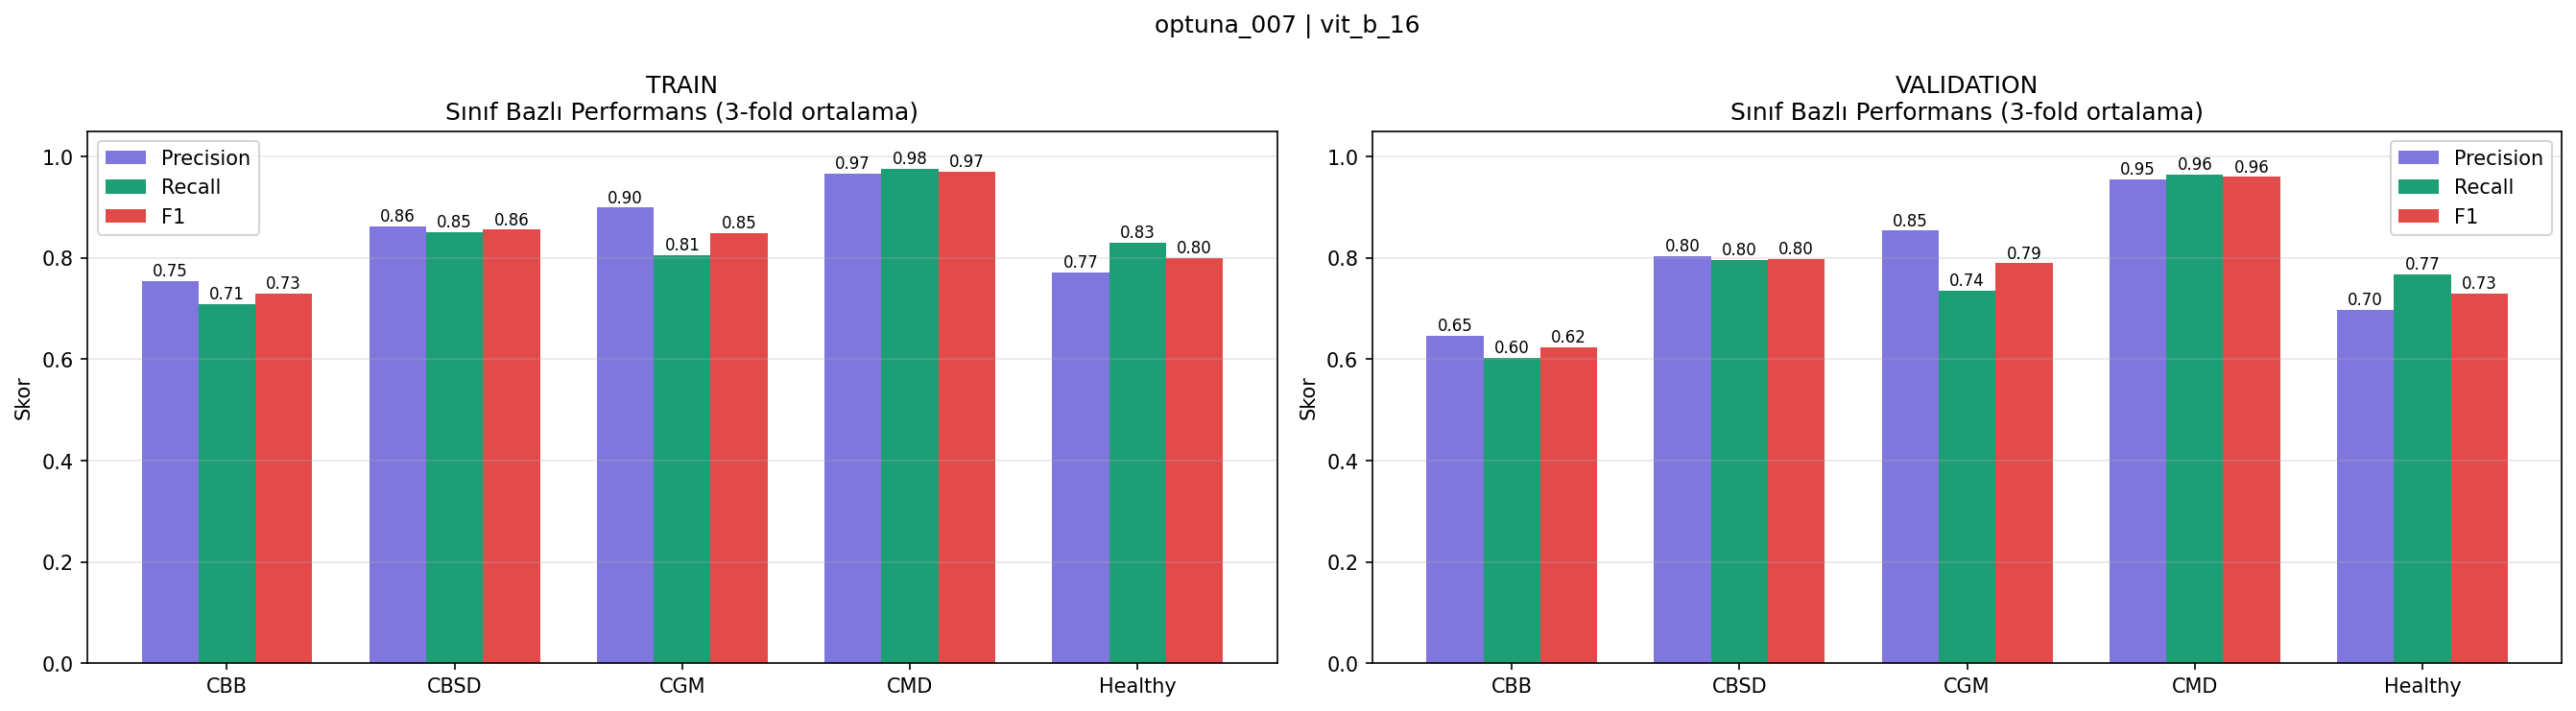
\includegraphics[width=\linewidth]{fig/fig_perclass_best_dl.png}
\caption{Per-class precision, recall, and F1 of the selected best deep-learning trial (mean across 3 folds). The model handles CMD almost perfectly ($F_1 \approx 0.96$) but is weakest on CBB ($F_1 \approx 0.63$), the rarest class.}
\label{fig:perclass}
\end{figure}

\begin{figure}[t]
\centering
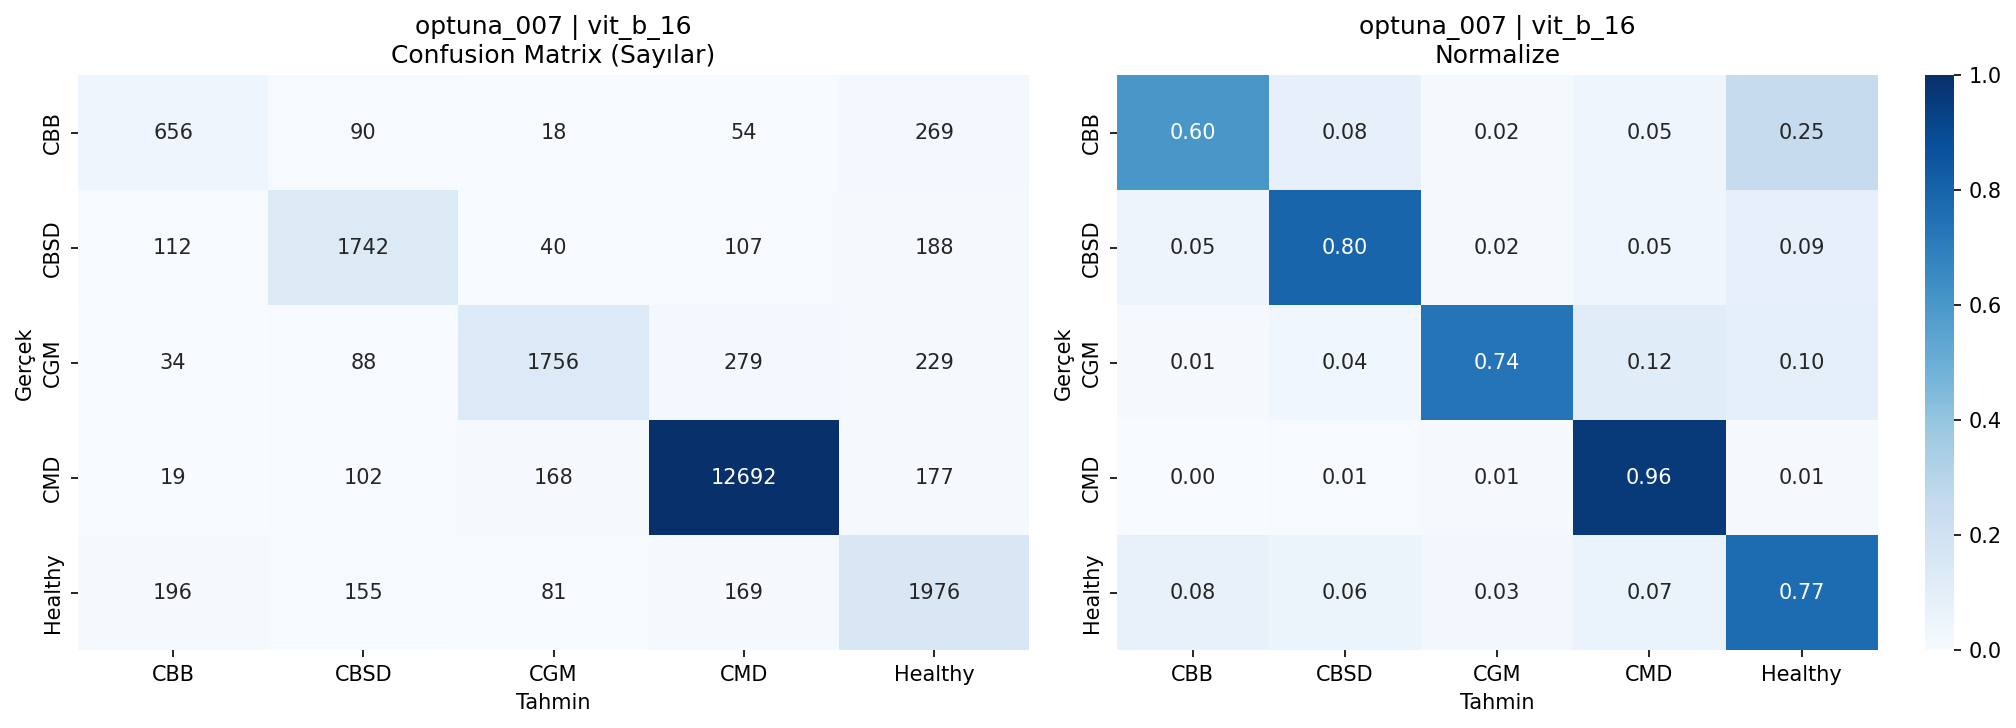
\includegraphics[width=\linewidth]{fig/fig_cm_best_dl.png}
\caption{Confusion matrix of the selected best deep-learning trial (out-of-fold predictions aggregated across 3 folds). Most off-diagonal mass for CBB and Healthy is absorbed into CMD, the dominant class.}
\label{fig:cm_best}
\end{figure}

\begin{figure}[t]
\centering
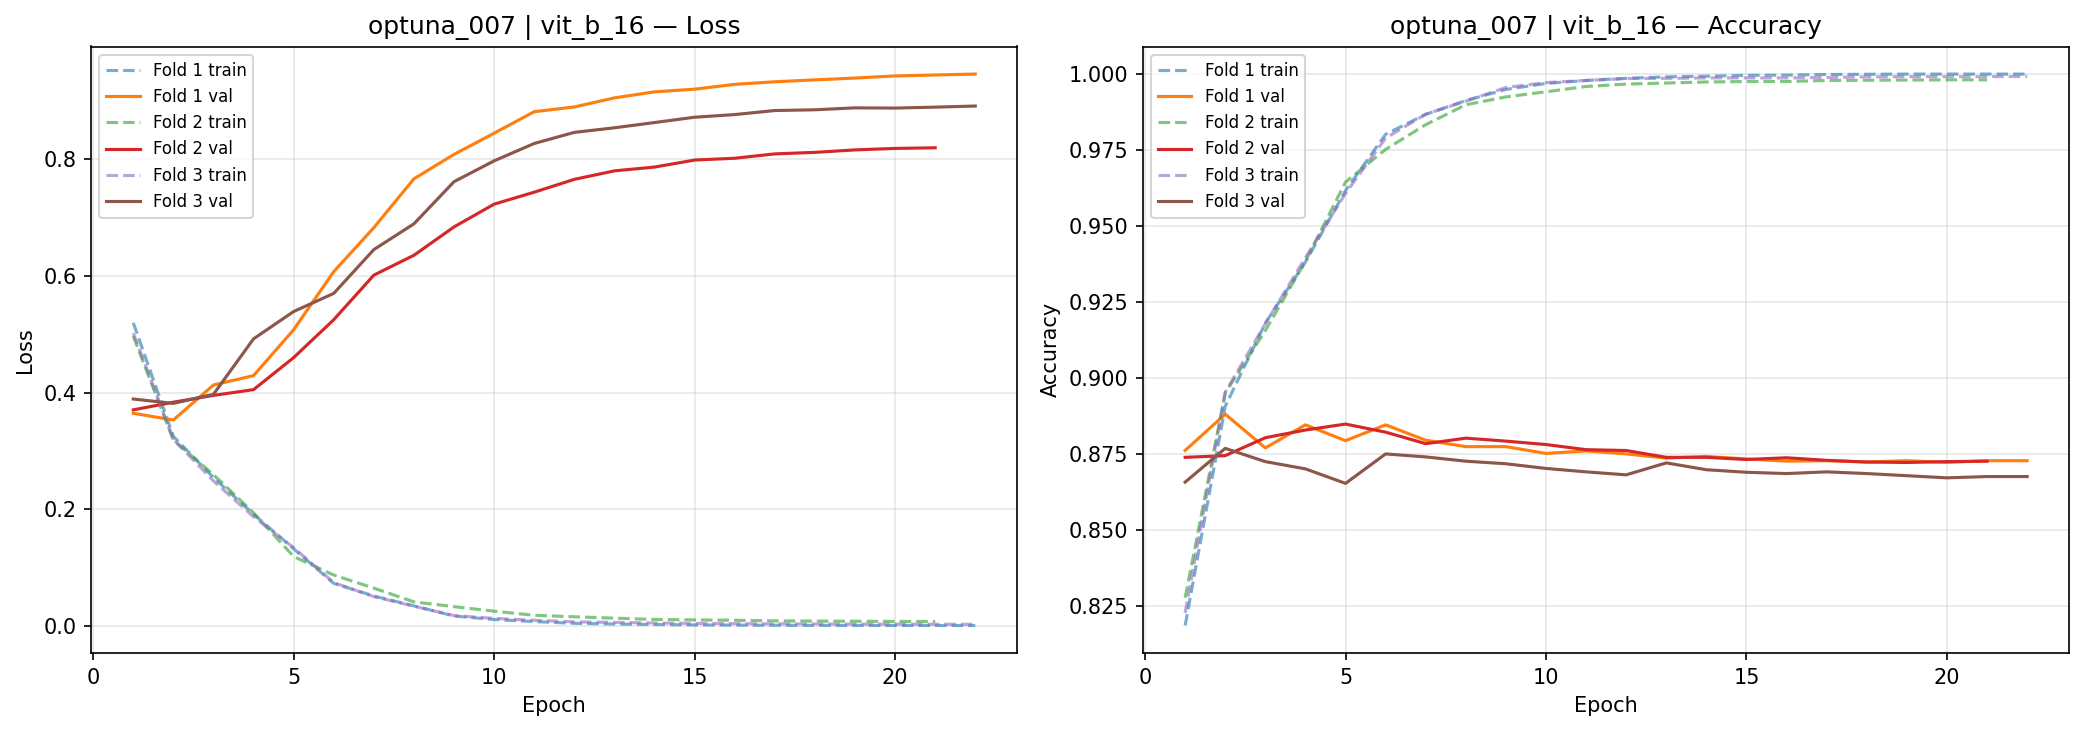
\includegraphics[width=\linewidth]{fig/fig_curves_best_dl.png}
\caption{Training and validation loss/accuracy curves for the selected best trial across the three folds. Convergence is extremely fast (best epoch within $[1,2]$ on every fold), after which validation loss diverges from training loss; the early-stopping criterion restores the best validation checkpoint before final evaluation.}
\label{fig:curves}
\end{figure}

A notable observation is that the best validation epoch falls in the range $[1, 2]$ on all three folds, despite the $200$-epoch budget and patience $20$. This indicates that fine-tuning a fully ImageNet-pretrained ViT on CLDC saturates extremely quickly: after roughly two epochs of full-network adaptation, additional epochs only increase the train--validation gap. The current best deep-learning trial reaches accuracy $\approx 0.88$, and targeted augmentation strategies reported in Section~\ref{ssec:results_aug} further reduce the train--validation gap and improve the macro objective.

\subsection{Per-Class Behavior and Hardest Class}
Across every leading trial in Tables~\ref{tab:results_cnn} and~\ref{tab:results_vit}, the per-class metrics follow the same pattern. CMD is essentially solved ($F_1 \approx 0.96$), CBSD and CGM reach the high $0.75$--$0.80$ range, Healthy lies near $0.72$, and CBB is consistently the hardest class with $F_1 \approx 0.63$ at best. Two factors are responsible. First, CBB has only $1{,}087$ training images (about one-twelfth of CMD), so even balanced reweighting cannot fully compensate for the limited intra-class diversity. Second, the visual symptoms of CBB (angular leaf spots) overlap with both Healthy and CGM under varying illumination, which puts a hard ceiling on the achievable per-class F1 without targeted augmentation. These observations directly motivate the augmentation ablation reported next.

\subsection{Augmentation Ablation}
\label{ssec:results_aug}
To quantify the effect of data augmentation independently of the hyperparameter search, the selected best ViT-B/16 configuration of Table~\ref{tab:best_dl} is held fixed and re-trained under $15$ augmentation settings, including the no-augmentation baseline. All other settings (learning rate, weight decay, batch size, optimizer, scheduler, class-weighting flag, seed, input resolution, epoch budget) are identical across runs, so any observed differences in validation metrics are attributable to the augmentation policy alone. The no-augmentation row in this ablation is a retrained baseline produced with the fixed ablation script, yielding macro-F1 $0.7812 \pm 0.0096$; this is close to the selected hyperparameter-search trial in Table~\ref{tab:best_dl} ($0.7800 \pm 0.0087$). Table~\ref{tab:results_aug} reports the full ranking and Fig.~\ref{fig:aug_bar} visualizes the results.

\begin{table*}[t]
\centering
\caption{Augmentation ablation results on CLDC. All trials use the selected best ViT-B/16 configuration from Table~\ref{tab:best_dl} as a fixed starting point; only the augmentation policy varies. Values are mean$\pm$std across 3 folds. ``$\Delta$F1'' is the change in macro-F1 with respect to the \texttt{none} baseline. Rows are ranked by macro-F1.}
\label{tab:results_aug}
\renewcommand{\arraystretch}{1.2}
\setlength{\tabcolsep}{4pt}
\begin{tabular}{clccccc}
\toprule
\textbf{Rank} & \textbf{Augmentation} & \textbf{F1 (macro)} & \textbf{Accuracy} & \textbf{Prec.\ (macro)} & \textbf{Recall (macro)} & \textbf{$\Delta$F1 vs none} \\
\midrule
\textbf{1} & \texttt{heavy\_combo} & \textbf{$0.7921 \pm 0.0068$} & \textbf{$0.8855 \pm 0.0040$} & \textbf{0.7980} & \textbf{0.7890} & \textbf{$+0.0109$} \\
2 & \texttt{cutout\_double} & $0.7888 \pm 0.0065$ & $0.8835 \pm 0.0031$ & 0.7923 & 0.7864 & $+0.0075$ \\
3 & \texttt{regularization\_light\_combo} & $0.7878 \pm 0.0075$ & $0.8843 \pm 0.0048$ & 0.8005 & 0.7786 & $+0.0065$ \\
4 & \texttt{comp\_3rd} & $0.7877 \pm 0.0040$ & $0.8835 \pm 0.0028$ & 0.7959 & 0.7821 & $+0.0064$ \\
5 & \texttt{comp\_resnext} & $0.7867 \pm 0.0060$ & $0.8844 \pm 0.0045$ & 0.8033 & 0.7749 & $+0.0054$ \\
6 & \texttt{comp\_vit} & $0.7866 \pm 0.0109$ & $0.8848 \pm 0.0039$ & 0.7995 & 0.7806 & $+0.0053$ \\
7 & \texttt{clahe\_enhanced} & $0.7854 \pm 0.0040$ & $0.8850 \pm 0.0016$ & 0.8041 & 0.7718 & $+0.0041$ \\
8 & \texttt{color\_light\_combo} & $0.7843 \pm 0.0036$ & $0.8832 \pm 0.0024$ & 0.7976 & 0.7728 & $+0.0030$ \\
9 & \texttt{contrast\_only} & $0.7835 \pm 0.0083$ & $0.8811 \pm 0.0058$ & 0.7929 & 0.7773 & $+0.0022$ \\
10 & \texttt{perspective\_light} & $0.7830 \pm 0.0087$ & $0.8828 \pm 0.0049$ & 0.7975 & 0.7719 & $+0.0018$ \\
11 & \texttt{flip\_only} & $0.7827 \pm 0.0038$ & $0.8818 \pm 0.0034$ & 0.7936 & 0.7746 & $+0.0014$ \\
12 & \texttt{color\_only} & $0.7819 \pm 0.0049$ & $0.8813 \pm 0.0030$ & 0.7985 & 0.7688 & $+0.0007$ \\
13 & \texttt{none} (baseline) & $0.7812 \pm 0.0096$ & $0.8800 \pm 0.0063$ & 0.7927 & 0.7740 & --- \\
14 & \texttt{blur\_noise\_light} & $0.7799 \pm 0.0063$ & $0.8814 \pm 0.0034$ & 0.7984 & 0.7654 & $-0.0013$ \\
15 & \texttt{rotate\_only} & $0.7775 \pm 0.0017$ & $0.8805 \pm 0.0022$ & 0.7934 & 0.7674 & $-0.0038$ \\
\bottomrule
\end{tabular}
\end{table*}


\begin{figure}[t]
\centering
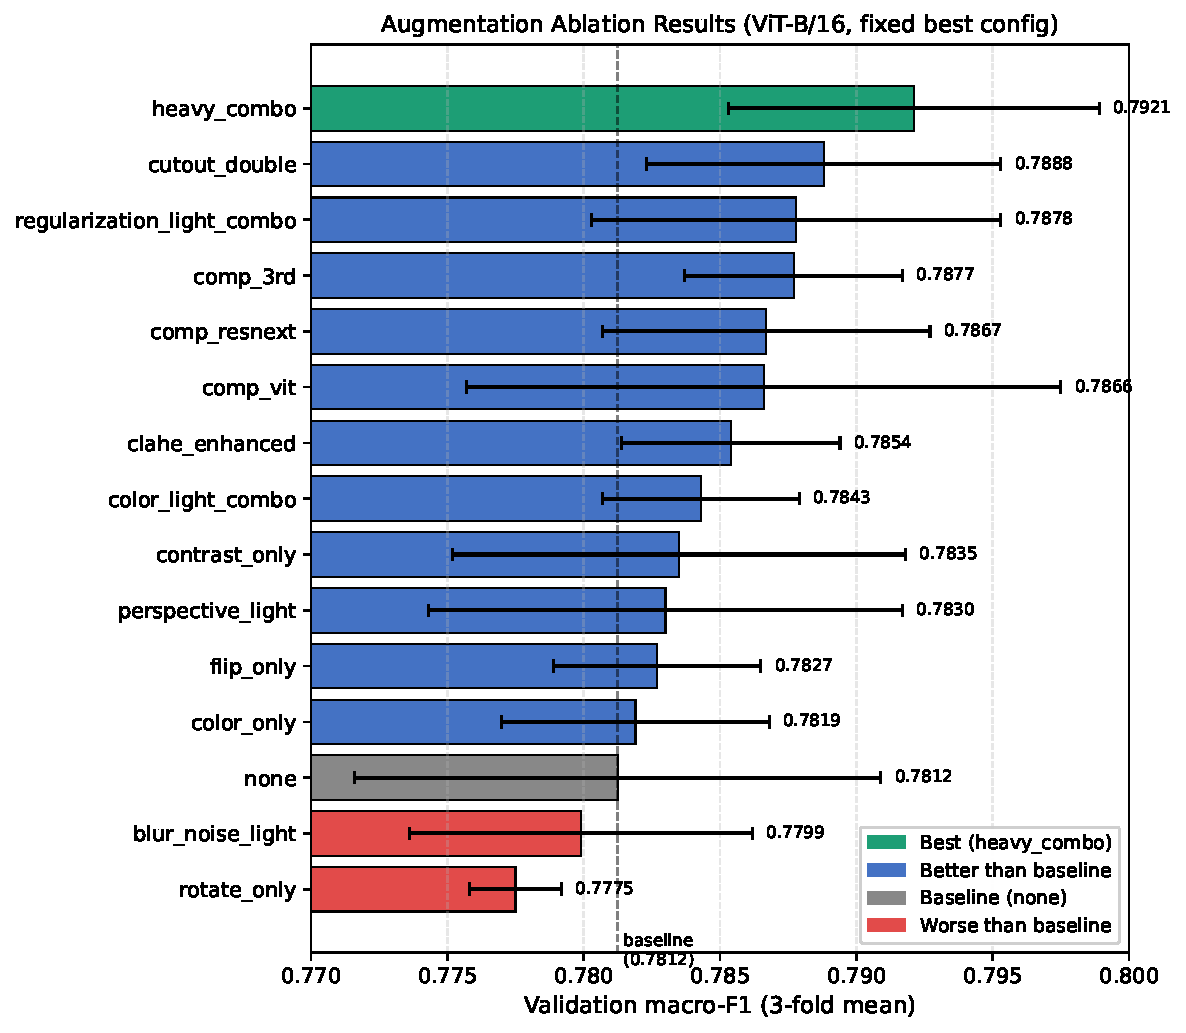
\includegraphics[width=\linewidth]{fig/fig_aug_comparison.pdf}
\caption{Augmentation ablation: validation macro-F1 of the selected best ViT-B/16 configuration under each augmentation policy. Error bars denote one standard deviation across the 3 folds. The dashed vertical line marks the \texttt{none} baseline; bars are colored to indicate whether each augmentation improved (blue), degraded (red), or matched (gray for baseline, green for best) the baseline performance.}
\label{fig:aug_bar}
\end{figure}

Several observations follow from these results. First, $12$ of the $14$ non-baseline augmentation policies (every entry except \texttt{blur\_noise\_light} and \texttt{rotate\_only}) outperform the no-augmentation baseline on macro-F1, which directly confirms the project hypothesis that data augmentation is beneficial on CLDC. Second, the largest gains come from combined policies that mix geometric, photometric, and occlusion-style transformations: \texttt{heavy\_combo} (rank $1$), \texttt{cutout\_double} (rank $2$), and \texttt{regularization\_light\_combo} (rank $3$) all combine multiple augmentation families and form the top of the table. Third, single-component policies that include only one weak transformation (e.g.\ \texttt{rotate\_only}, \texttt{blur\_noise\_light}) actually reduce macro-F1 relative to baseline, showing that weak, isolated augmentations can act as noise without compensating regularization benefits. Fourth, the train--validation gap of the best augmentation ($0.0396$ for \texttt{heavy\_combo}) is meaningfully smaller than that of the no-augmentation baseline ($0.0604$), indicating that augmentation reduces overfitting rather than simply shifting the operating point.

\subsubsection{Selected Best Augmentation: \texttt{heavy\_combo}}
The best augmentation policy is \texttt{heavy\_combo}, with macro-F1 $0.7921 \pm 0.0068$ and accuracy $0.8855 \pm 0.0040$. This corresponds to an absolute improvement of $+0.0109$ macro-F1 over the no-augmentation baseline (a $+1.4\%$ relative gain), achieved while simultaneously reducing the train--validation gap from $0.0604$ to $0.0396$ and pushing the best-epoch range from $[1,2]$ in the baseline to $[7,11]$ across folds, which indicates that the model is now able to make productive use of the additional training budget rather than overfitting after one or two epochs. The combination of full geometric transformations, full color jittering, and Random Erasing therefore acts both as a regularizer (reducing the train--validation gap) and as a data-diversity amplifier (extending useful training time).

\begin{figure*}[t]
\centering
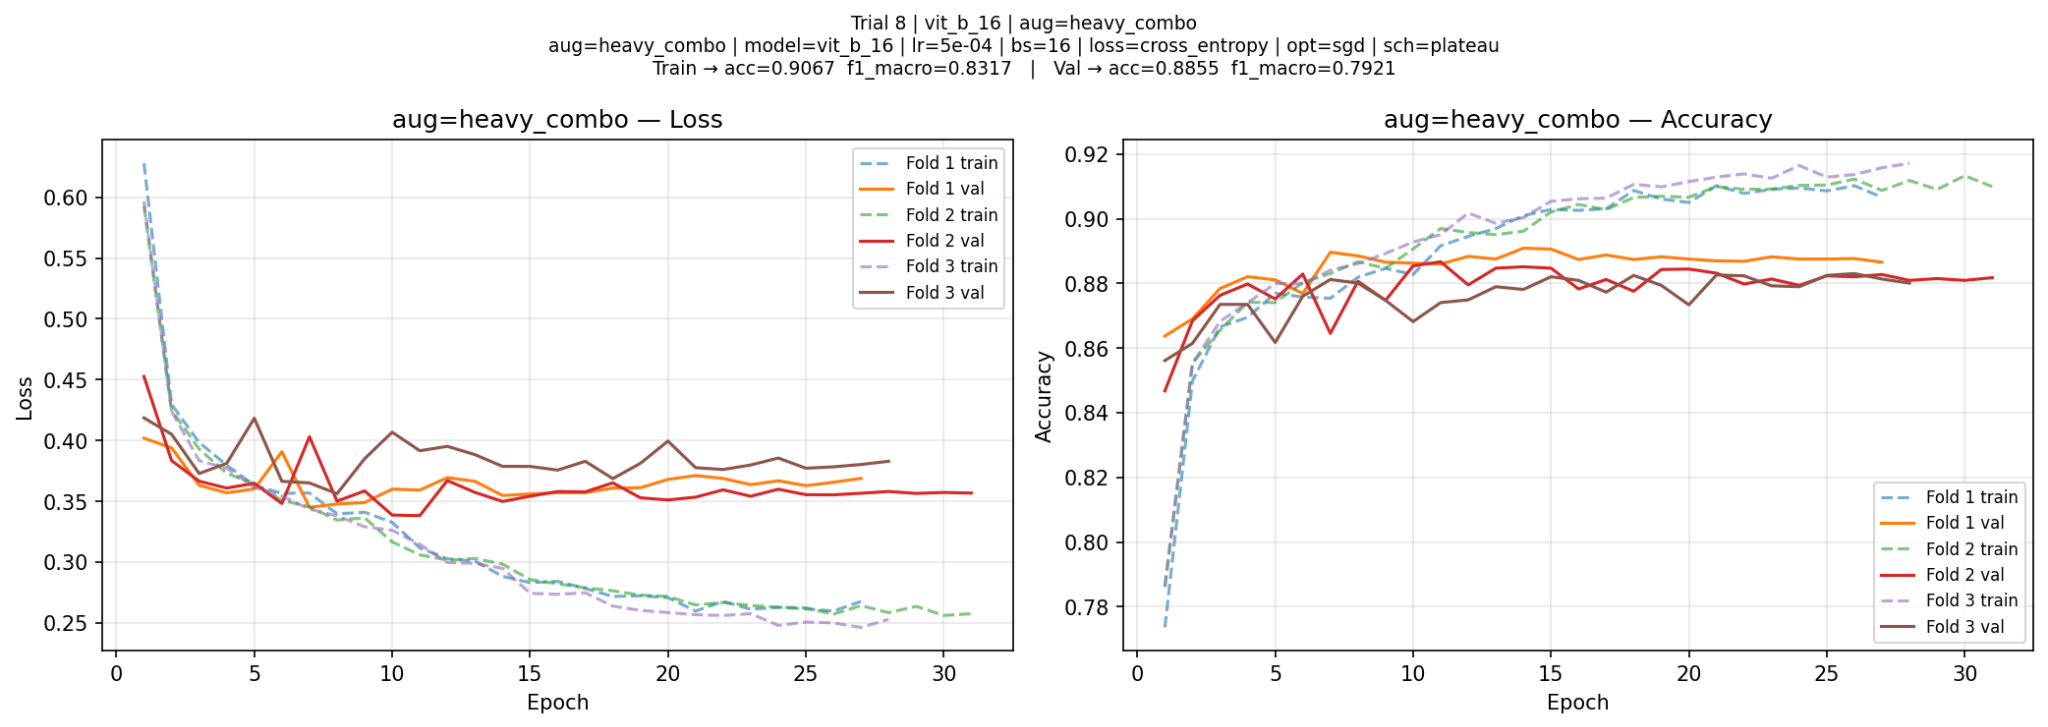
\includegraphics[width=1.04\textwidth]{fig/fig_curves_aug_heavy_combo.png}
\caption{Training and validation curves for the selected best augmentation policy, \texttt{heavy\_combo}, using the same ViT-B/16 configuration as the no-augmentation baseline. In contrast to Fig.~\ref{fig:curves}, training loss no longer collapses to zero and validation loss no longer diverges upward after the first few epochs. The curves instead show slower training convergence, validation-loss stabilization around the mid-$0.3$ range, and validation accuracy near $88$--$89\%$ across folds.}
\label{fig:curves_aug_heavy}
\end{figure*}

Figure~\ref{fig:curves_aug_heavy} explains the mechanism behind the augmentation gain by comparing directly with the pre-augmentation curves in Fig.~\ref{fig:curves}. Without augmentation, the model memorizes the training folds rapidly: training loss approaches zero, training accuracy approaches $100\%$, validation loss rises monotonically after the first few epochs, and validation accuracy saturates around $87$--$88\%$. With \texttt{heavy\_combo}, training remains deliberately harder: training loss decreases more slowly and remains around $0.25$ at the end of training, while training accuracy stabilizes near $91\%$ instead of reaching perfect memorization. More importantly, validation loss stays approximately stable around $0.35$--$0.38$ rather than increasing toward $0.8$--$0.9$, and validation accuracy remains in the $88$--$89\%$ band. This behavior confirms that the augmentation policy improves generalization by suppressing memorization and by keeping the optimization trajectory useful for more epochs, rather than by merely increasing the apparent validation accuracy at a single early checkpoint.

\begin{figure}[t]
\centering
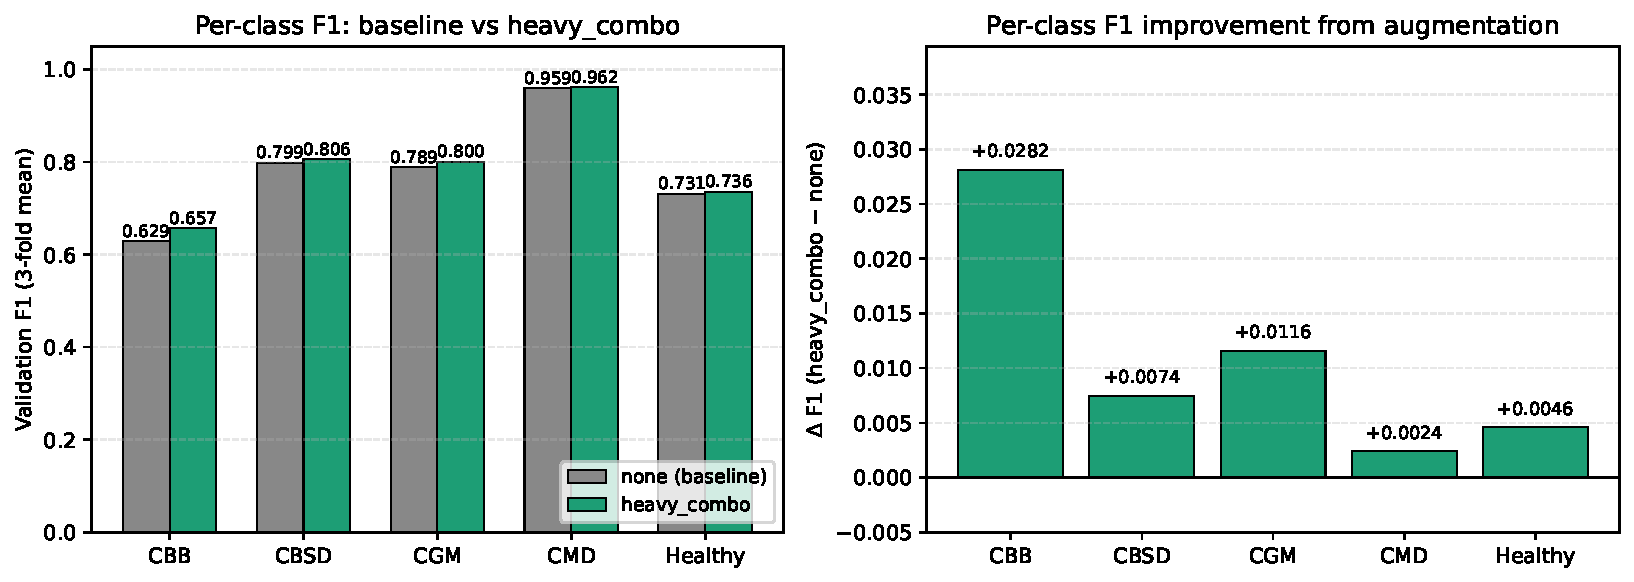
\includegraphics[width=\linewidth]{fig/fig_perclass_delta.pdf}
\caption{Per-class effect of the best augmentation policy. Left: per-class validation F1 under the no-augmentation baseline (gray) and under \texttt{heavy\_combo} (green). Right: per-class change $\Delta F_1$ from baseline to \texttt{heavy\_combo}; all five classes improve, and the largest gain ($+0.0282$) is on the rarest and previously hardest class, CBB.}
\label{fig:aug_perclass_delta}
\end{figure}

The per-class behavior of \texttt{heavy\_combo} (Fig.~\ref{fig:aug_perclass_delta}) is the most informative aspect of the augmentation ablation. All five classes gain F1, but the gains are highly asymmetric: CBB, the rarest class and the one with the lowest baseline F1, gains the most ($+0.0282$ F1), followed by CGM ($+0.0116$) and CBSD ($+0.0074$). The two best-performing classes at baseline (CMD with $F_1 \approx 0.96$ and Healthy with $F_1 \approx 0.73$) gain the least ($+0.0024$ and $+0.0046$ respectively). This is the desired pattern for an imbalanced dataset: augmentation reallocates the model's representational capacity toward the harder, minority class without sacrificing performance on the majority class.

\begin{figure*}[t]
\centering
\begin{tabular}{cc}
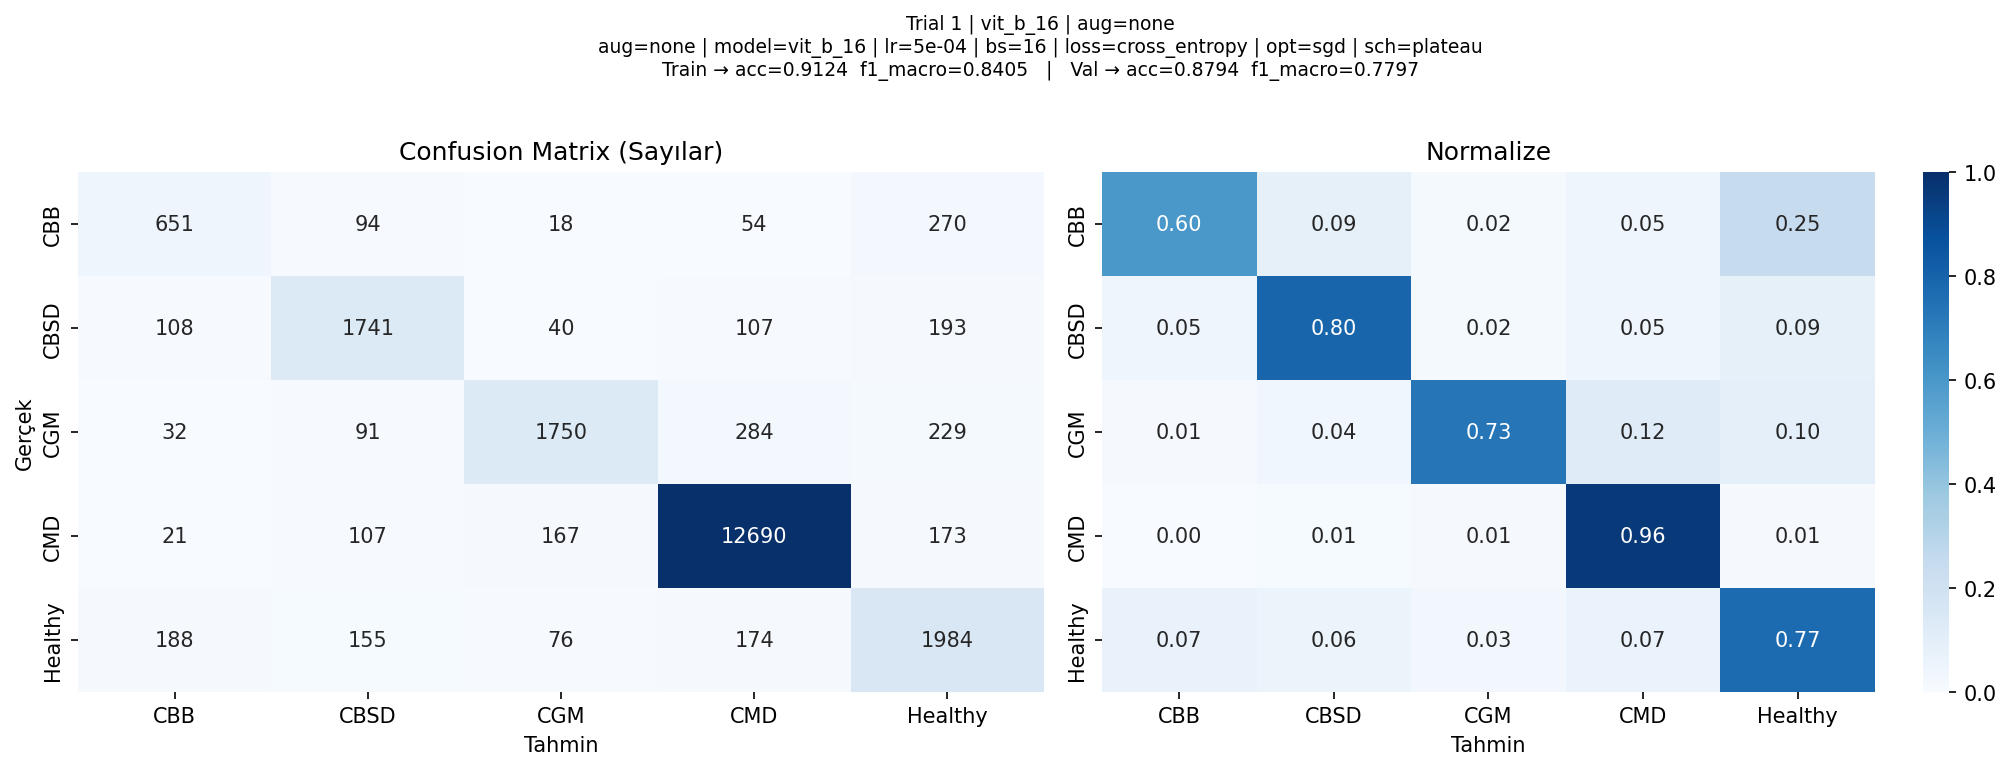
\includegraphics[width=0.46\linewidth]{fig/fig_cm_aug_none.png} &
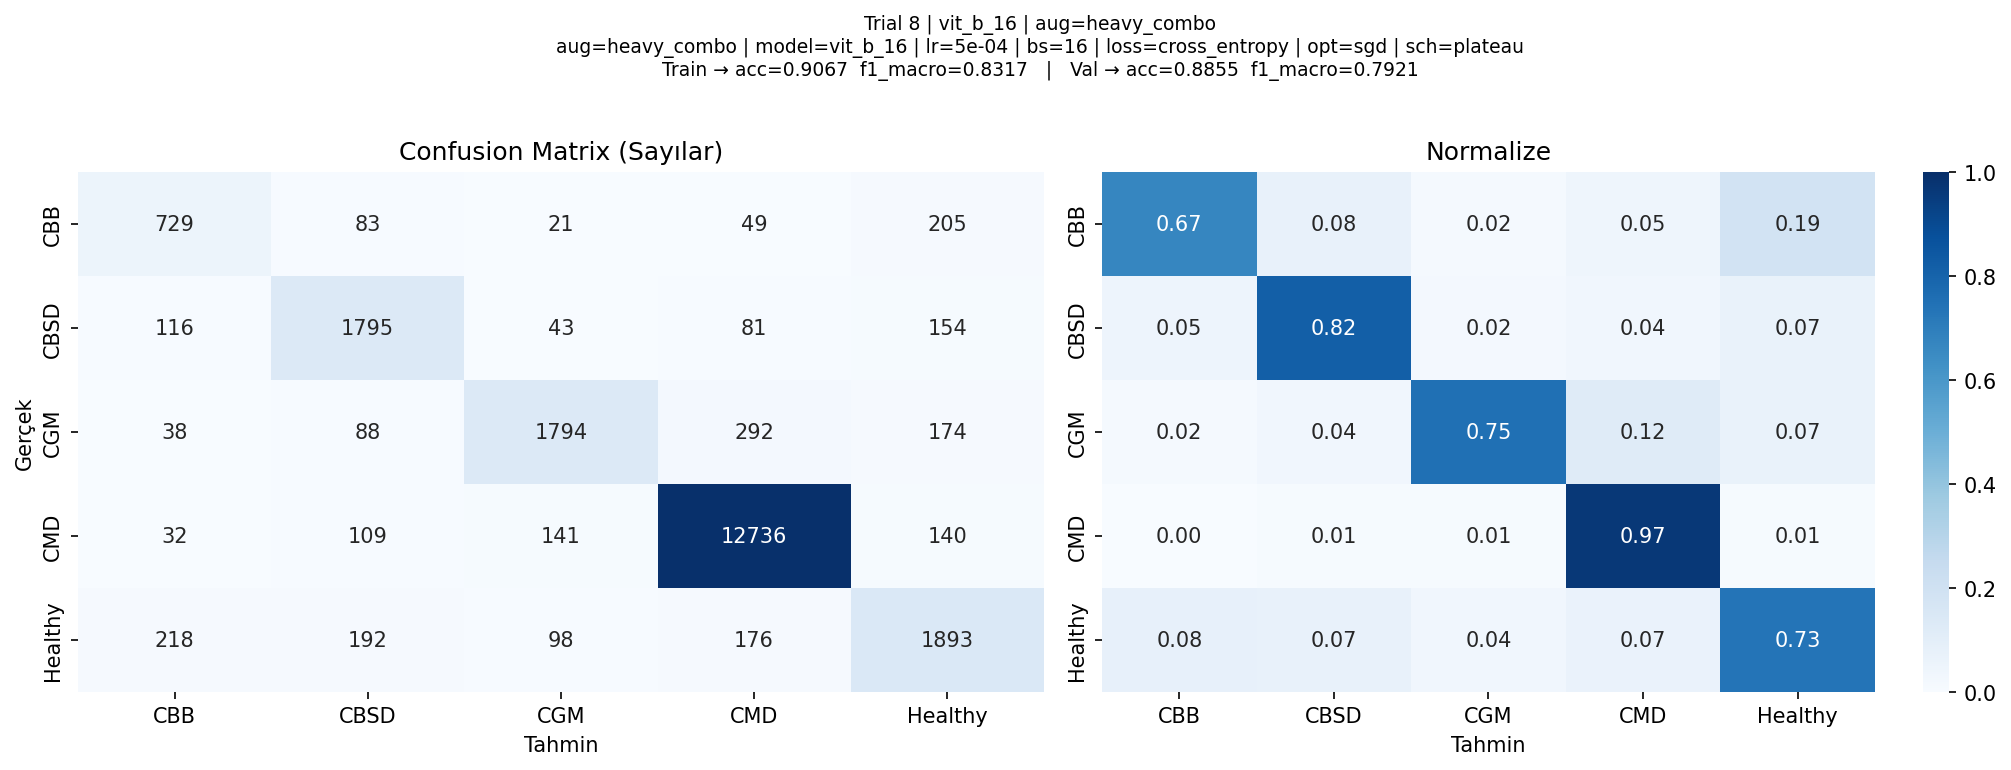
\includegraphics[width=0.46\linewidth]{fig/fig_cm_aug_heavy.png} \\
(a) \texttt{none} (baseline) & (b) \texttt{heavy\_combo} (best) \\
\end{tabular}
\caption{Out-of-fold confusion matrices for the no-augmentation baseline (a) and the best augmentation policy \texttt{heavy\_combo} (b), both evaluated with the selected best ViT-B/16 configuration. The reduction of off-diagonal mass for CBB and CBSD (rows~$0$ and $1$) is the dominant source of the macro-F1 improvement.}
\label{fig:cm_aug}
\end{figure*}

The confusion matrices in Fig.~\ref{fig:cm_aug} make the per-class effect concrete. Under the no-augmentation baseline the model confuses CBB with CMD and CGM relatively often, and CBSD with CMD; \texttt{heavy\_combo} reduces both off-diagonal blocks. The dominant diagonal cell for CMD remains essentially unchanged, confirming that the majority class is unaffected by the augmentation.

% =====================================================================
% Discussion and Conclusion
% =====================================================================

\section{Discussion and Conclusion}
\label{sec:discussion}

\begin{table*}[t]
\centering
\caption{Comparison with publicly documented Kaggle CLDC solutions. Reported leaderboard/test results are not strictly identical to our 3-fold CV because the Kaggle systems generally use external data, TTA, ensembling, relabeling, or hidden-test model selection. ``pp'' denotes percentage points relative to our best post-augmentation accuracy of $88.55\%$.}
\label{tab:kaggle_comparison}
\footnotesize
\setlength{\tabcolsep}{2.5pt}
\begin{tabular}{p{0.14\linewidth} p{0.22\linewidth} p{0.17\linewidth} p{0.18\linewidth} p{0.18\linewidth}}
\toprule
Work & Main setup & Validation / selection & Reported best result & Difference vs. ours \\
\midrule
lizh0019 / golddiggaz~\cite{lizh0019cassava} & Ensemble of EfficientNet-B4, ResNeXt50, ViT, and MobileNet/CropNet-style models & OOF ensemble search; competition selection & $\approx 91.3\%$ public/private LB, rank 1 & $+2.75$ pp vs. our $88.55\%$ CV accuracy \\
Devon Stanfield~\cite{devonstanfield2021cassava} & TensorFlow Hub CropNet cassava classifier inference notebook & Public notebook; leaderboard selection & $90.43\%$ private LB, rank 2 in available snapshot & $+1.88$ pp; method details less complete \\
TomYanabe~\cite{tomyanabe2021cassava} & ViT-B/16 at 224/384 input resolutions, 2020+2019 data, TTA=5 & 5-fold StratifiedKFold & CV $90.75\%$, public $90.75\%$, private $90.28\%$, rank 3 & $+1.73$ pp; closest high-rank k-fold comparison \\
Krut Patel~\cite{krutpatel2021cassava} & ResNeXt50-32x4d + EfficientNet-B4 soft-voting ensemble with TTA & Stratified k-fold CV & $89.5\%$ public/private LB, rank 9 & $+0.95$ pp; similar k-fold design but ensemble/TTA used \\
Kozodoi~\cite{kozodoi2021cassava} & CNN + Vision Transformer stacking ensemble & Base-model training plus stacking & $91.06\%$ reported test accuracy, top 1\% / rank 14 & $+2.51$ pp; ensemble and stacking not used here \\
kqu7~\cite{kqu7cassava} & ResNeXt50 + EfficientNet variants, class sampling, heavy augmentation, 8x TTA & 5-fold StratifiedKFold & CV $89.3$--$89.8\%$; public $90.11\%$, private $90.01\%$ & $+1.46$ pp on private LB; very close protocol but ensemble/TTA used \\
This work & Single ViT-B/16 with Optuna-selected hyperparameters and \texttt{heavy\_combo} augmentation & 3-fold StratifiedKFold & Accuracy $88.55\% \pm 0.40\%$, macro-F1 $0.7921 \pm 0.0068$ & Baseline for controlled single-model study \\
\bottomrule
\end{tabular}
\end{table*}

This work presented a controlled, reproducibility-oriented comparison of three families of image classification approaches for the Cassava Leaf Disease Classification benchmark---classical machine-learning baselines, two convolutional architectures (ResNet-50, EfficientNet-B4), and the Vision Transformer (ViT-B/16)---together with an Optuna-driven categorical hyperparameter search and an augmentation ablation. We organize the discussion around five findings that emerge from the experiments and from the comparison with public Kaggle solutions.

\paragraph{Architecture matters, but less than expected at scale}
Among the deep architectures, ViT-B/16 produces the strongest results: every entry in the ViT top-10 (Table~\ref{tab:results_vit}) surpasses the best ResNet-50 trial in Table~\ref{tab:results_cnn}, and the absolute gap between the best ViT trial ($0.7803$ macro-F1) and the best CNN trial ($0.7405$ macro-F1) is approximately $+0.04$ macro-F1, or about $5\%$ relative. This is a substantial margin given the difficulty of the dataset and is consistent with the broader literature showing that ImageNet-pretrained transformers transfer well to natural-image tasks. However, the gap between the two CNN backbones is much smaller and not monotonic: nine of the top-10 CNN trials use ResNet-50 and the best EfficientNet-B4 trial appears only at rank $9$, suggesting that the larger compound-scaled architecture does not consistently outperform the simpler ResNet baseline at the hyperparameter budgets we explored. In practice this means that for a given compute budget, the choice between competitive CNN backbones is dominated by hyperparameter and augmentation choices rather than by architectural depth or scaling alone. Input resolution differs across architectures; part of the ViT advantage may be attributable to higher resolution.

\paragraph{Classical baselines are inadequate on raw pixels}
The classical pipeline (grayscale $64{\times}64$ flatten $\rightarrow$ StandardScaler $\rightarrow$ PCA at $95\%$ variance $\rightarrow$ classifier) yields macro-F1 scores below $0.21$ across all four classifiers (Table~\ref{tab:results_ml}), more than $0.53$ macro-F1 points below the best deep model. Tree-based methods reach an apparently high accuracy ($\approx 0.6149$) only because they collapse to predicting the majority CMD class on almost every example, as evidenced by their degenerate per-class precision and recall. This confirms that the discriminative cues for CLDC live in fine-grained local leaf texture rather than in global pixel statistics, and that any reasonable classifier on raw pixels alone cannot solve this task.

\paragraph{Hyperparameter choices and class weighting}
The Optuna search reveals two consistent patterns. First, the top deep-learning trials come from the combined search over both class-weighted and unweighted configurations; the CW column in Tables~\ref{tab:results_cnn} and~\ref{tab:results_vit} makes this explicit. The highest-ranked models are dominated by unweighted training (eight of ten ViT trials, nine of ten CNN trials), while class-weighted candidates generally trade minority-class recall for majority-class precision rather than improving the macro objective monotonically. Second, on this dataset the best ViT configurations consistently used SGD with Nesterov momentum and a plateau or cosine warm-restart schedule rather than AdamW, despite AdamW being the de-facto default for transformer fine-tuning. We interpret this as a property of the dataset rather than a property of the architecture: with strongly imbalanced labels and noisy real-world images, the implicit regularization of SGD appears to outperform the more aggressive adaptation of AdamW. A practical consequence is that for similar agricultural in-the-wild benchmarks, hyperparameter assumptions imported from clean academic datasets should be questioned and re-tuned.

\paragraph{Augmentation gains concentrate on the minority class}
The augmentation ablation reported in Section~\ref{ssec:results_aug} is, in our view, the most informative experiment in this work. Twelve of the fourteen non-baseline augmentation policies improve macro-F1 over the no-augmentation baseline (Table~\ref{tab:results_aug}), the best policy (\texttt{heavy\_combo}) achieves macro-F1 $0.7921 \pm 0.0068$ versus the baseline's $0.7812 \pm 0.0096$, and the per-class breakdown in Fig.~\ref{fig:aug_perclass_delta} shows that the largest absolute gain ($+0.0282$ F1) is on CBB, the rarest and previously hardest class, while the majority CMD class is essentially unaffected ($+0.0024$ F1). The training curves make the same conclusion visible at the optimization level: Fig.~\ref{fig:curves} shows near-immediate memorization without augmentation, whereas Fig.~\ref{fig:curves_aug_heavy} shows that \texttt{heavy\_combo} slows down training convergence, prevents the validation-loss explosion, and keeps validation accuracy stable for a longer useful training window. The train--validation gap drops from $0.0604$ to $0.0396$, and the best-epoch indices move from $[1,2]$ on the baseline to $[7,11]$ on \texttt{heavy\_combo}, indicating that augmentation both reduces overfitting and allows the model to make productive use of additional training time. In contrast, single-component policies that include only one weak transformation can reduce macro-F1 below baseline (\texttt{rotate\_only}, \texttt{blur\_noise\_light}), which suggests that effective augmentation requires combining multiple augmentation families rather than relying on a single transformation.

\paragraph{Comparison with Kaggle competition systems}
Table~\ref{tab:kaggle_comparison} places our best post-augmentation model against publicly documented Kaggle CLDC solutions. The strongest leaderboard systems remain above our result, but the gap is methodologically expected. Their improvements come from system-level competition techniques: ensembling multiple backbones, using 2019/external cassava data, training fold ensembles, applying TTA, relabeling noisy samples, or stacking OOF predictions. In contrast, our final model is a single ViT-B/16 trained under a fixed 3-fold protocol. The most comparable k-fold solutions are TomYanabe, Krut Patel, and kqu7. They exceed our accuracy by about $0.95$--$1.73$ percentage points, but all three use ensembles and/or TTA. This comparison suggests that our post-augmentation single-model result is close to the lower end of competitive Kaggle-era performance, while the remaining performance gap is largely attributable to ensemble-scale inference and additional data rather than to the absence of a fundamentally different backbone.



\paragraph{Limitations and future work}
Three limitations of the present work are worth stating explicitly. First, we evaluate exclusively under 3-fold stratified cross-validation and do not use a separately held-out test split; out-of-fold validation predictions are reported as a proxy for held-out test performance. While this is statistically meaningful, a fixed external test split would allow a more rigorous comparison with published numbers. Second, the augmentation ablation is conducted on top of a single selected ViT-B/16 configuration; we have not verified whether the same ranking of augmentation policies would hold under other backbones or under significantly different optimizer/scheduler combinations. Third, the input resolution differs across architectures: ResNet-50 and EfficientNet-B4 use $224{\times}224$, whereas ViT-B/16 uses $384{\times}384$, so part of the ViT advantage may be attributable to higher resolution. Fourth, the experiments are run with single-seed fine-tuning rather than seed averaging, so the reported macro-F1 values include some seed-level variance that we did not characterize. Promising directions for follow-up work include (i)~combining the best augmentation policy with light test-time augmentation, (ii)~revisiting class-imbalance handling under augmentation, and (iii)~adding model-ensemble or distillation steps on top of the Optuna-selected best configurations.

\paragraph{Conclusion}
Within a unified evaluation protocol and a categorical hyperparameter search, ViT-B/16 fine-tuned from ImageNet weights is the strongest single-model approach on CLDC among the configurations we evaluated, reaching macro-F1 $0.7921 \pm 0.0068$ and accuracy $0.8855 \pm 0.0040$ when combined with the best augmentation policy (\texttt{heavy\_combo}). Classical pipelines on raw pixel statistics are not competitive on this benchmark. Across deep architectures, augmentation and hyperparameter choices contribute as much to the final performance as the choice of backbone, and the gains from augmentation are concentrated where they are most needed---on the minority class. Relative to public Kaggle systems, our result is best interpreted as a controlled single-model baseline: below leaderboard ensembles, but close enough to indicate that much of the gap can plausibly be closed by TTA, fold ensembling, relabeling, and additional data rather than by changing the basic ViT backbone.

% =====================================================================
% Bibliography
% =====================================================================
\bibliographystyle{IEEEtran}
\bibliography{references}

\end{document}
